%%
%% Copyright 2019-2020 Elsevier Ltd
%%
%% This file is part of the 'CAS Bundle'.
%% --------------------------------------
%%
%% It may be distributed under the conditions of the LaTeX Project Public
%% License, either version 1.2 of this license or (at your option) any
%% later version.  The latest version of this license is in
%%    http://www.latex-project.org/lppl.txt
%% and version 1.2 or later is part of all distributions of LaTeX
%% version 1999/12/01 or later.
%%
%% The list of all files belonging to the 'CAS Bundle' is
%% given in the file `manifest.txt'.
%%
%% Template article for cas-dc documentclass for
%% double column output.

%\documentclass[a4paper,fleqn,longmktitle]{cas-dc}
\documentclass[a4paper,fleqn]{cas-dc}

%\usepackage[authoryear,longnamesfirst]{natbib}
%\usepackage[authoryear]{natbib}
\usepackage[numbers]{natbib}

%%%Author definitions
\def\tsc#1{\csdef{#1}{\textsc{\lowercase{#1}}\xspace}}
\tsc{WGM}
\tsc{QE}
\tsc{EP}
\tsc{PMS}
\tsc{BEC}
\tsc{DE}
%%%

%插入伪代码
\let\classAND\AND
\let\AND\relax
% load algorithmic
\usepackage{algorithmic}
\usepackage{algorithm}
\usepackage{subfig}

% save the new meaning of \AND and restore one of the class
\let\algoAND\AND
\let\AND\classAND
% but when we start \begin{algorithmic} we want its own \AND
\AtBeginEnvironment{algorithmic}{\let\AND\algoAND}

% \floatname{algorithm}{Algorithm}
\renewcommand{\algorithmicrequire}{\textbf{Input:}}
\renewcommand{\algorithmicensure}{\textbf{Output:}}
\renewcommand{\algorithmicendif}{\textbf{end}}


%调整断字
\hyphenpenalty=6000
\tolerance=700
\setlength{\emergencystretch}{2em}

%表格不要太宽
\usepackage{graphicx}
\usepackage{float}
\usepackage{multicol}
\usepackage{url}
%表格斜线
\usepackage{diagbox}

\newdefinition{definition}{Definition}
\newtheorem{theorem}{Theorem}
\newtheorem{remark}{Remark}

\begin{document}




\let\WriteBookmarks\relax
\def\floatpagepagefraction{1}
\def\textpagefraction{.001}
\shorttitle{Surface--Subsurface
Observation of Tropical Cyclones}
\shortauthors{Yihui Ding et~al.}

\title [mode = title]{%
\texorpdfstring{Multi-Agent Reinforcement Learning for
Surface--Subsurface Observation of Tropical Cyclones Using Submersible
Unmanned Vessels}%
{Multi-Agent Reinforcement Learning for Surface--Subsurface Observation of
Tropical Cyclones Using Submersible Unmanned Vessels}}
% \tnotemark[1,2]

% \tnotetext[1]{}

% \tnotetext[2]{}



\author[1,2]{Yihui Ding}[orcid=0009-0009-4133-1571]
\fnmark[1] % 添加脚注标记 1
\author[1,2,3]{\hspace*{0.33em}Xiwen Ma}[orcid=0000-0001-9212-3523]
\fnmark[1] % 添加脚注标记 1
\author[1,2]{\hspace*{0.33em}Wenlei Peng}
\author[1,2]{\hspace*{0.33em}Fangzheng Qi}[orcid=0009-0008-5974-7447]
\author[1,2,4]{\hspace*{0.33em}Jingsong Yang}[orcid=0000-0002-7514-3212]
\cormark[1]

\address[1]{School of Oceanography, Shanghai Jiao Tong University, Shanghai, 200030, China}
\address[2]{State Key Laboratory of Satellite Ocean Environment Dynamics, Second Institute of Oceanography, Ministry of Natural Resources, Hangzhou, 310012, China}
\address[3]{Institute of Automation Chinese Academy of Sciences, Beijing, 100190, China}
\address[4]{Southern Marine Science and Engineering Guangdong Laboratory (Zhuhai), Zhuhai, 519082, China}
\fntext[1]{These authors contributed equally to this work.}
\cortext[1]{Corresponding author: Jingsong Yang. Email:
\texttt{jsyang@sio.org.cn}}
\hypersetup{
  pdfauthor={Yihui Ding, Xiwen Ma, Wenlei Peng, Fangzheng Qi, Jingsong Yang},
  pdfsubject={Surface--subsurface tropical-cyclone observation with SUVs},
  pdfkeywords={tropical cyclone observation, cooperative task, submersible
    unmanned vessel, multi-agent reinforcement learning,
    surface--subsurface observation}
}

\begin{abstract}
Tropical cyclones are destructive, while intensity and rapid-intensification
forecasts remain limited by sparse near-core observations. Conventional
platforms rarely combine rapid transit with surface-wind and
subsurface-current sensing. Blue Whale-class submersible unmanned vessels can
transit rapidly at the surface to TC cores, then dive to observe temperature,
salinity, currents, and biogeochemical variables. We use simulation-based
multi-agent reinforcement learning for autonomous observation and
navigation. The environments combine ERA5 10 m winds and HYCOM currents from 0 to
60 m with IBTrACS tracks for 400 western North Pacific TCs. A
shared-observation independent proximal policy optimization (IPPO) policy
outputs one joint formation action for all surface SUVs and maps local current
histories to in-vehicle commands underwater at 10 min intervals. Surface
SUVs therefore share observations and preserve their initial relative
positions exactly; subsurface SUVs use only local current histories. We compare
12 m/s surface and 1.5 m/s submerged limits, close to current Blue Whale
design speeds, with 20 m/s and 2.0 m/s as future upgrades. Compared with four
traditional planners at surface experiments, the IPPO policy achieves the
lowest final tracking error, which means that the SUVs can reach
the TC core region more readily and obtain more valuable observations. For the
surface IPPO policy, we further evaluate ring,
line, grid, and V-shaped formations. After reaching the TC core region, the
SUVs dive vertically to different depths from 0 to 60 m for further
observations. Underwater, IPPO attains the largest geometric and
current-weighted coverage, while the potential field algorithm attains the
highest mean experienced current. Limitations remain that training and
validation are conducted in a simulation environment built from historical
reanalysis data; real-vehicle experiments are not included and require future
work.
\end{abstract}

% \begin{graphicalabstract}
% \includegraphics{figs/grabs.pdf}
% \end{graphicalabstract}

\begin{highlights}
\item Dual-mode SUVs track surface winds and sample subsurface variables.
\item Historical atmosphere--ocean environments cover 400 TCs in the western
North Pacific.
\item Parameter-sharing IPPO is trained for TC observation with 4--16 SUVs.
\item Comparison between MARL and traditional path-planning algorithms at both
stages.
\end{highlights}

\begin{keywords}
tropical cyclone observation \sep cooperative task \sep submersible unmanned vessel \sep
multi-agent reinforcement learning \sep
surface--subsurface observation
\end{keywords}

\maketitle

\section{Introduction}
Tropical cyclones (TCs) threaten coastal communities, infrastructure, and
offshore operations. Climate assessments indicate that some TC changes are
detectable despite observational uncertainty \citep{r1} and project an
increasing proportion of very intense TCs under continued warming \citep{r2},
while global TC frequency may decline \citep{r3} and rapid-intensification
events have recently increased in offshore regions \citep{r4}. Landfalling TCs
over the western North Pacific and China have also become more destructive,
with increasing nearshore intensification and exposure \citep{r5,r6,r7,r8}.
Track forecasts have improved substantially, but intensity prediction remains
more difficult: recent intensity guidance has reduced errors \citep{r9}, yet
official forecasts in the western North Pacific continue to carry substantial
uncertainty \citep{r10}. A central reason is that intensity depends on air--sea
enthalpy and momentum exchange, upper-ocean heat content, barrier layers,
mesoscale eddies, and TC-induced currents \citep{r11,r12}.

Existing observing platforms each cover only part of this problem. Spaceborne
microwave sensors provide broad but complementary and incomplete views of the
near-core wind field. Active scatterometers infer surface wind from ocean
backscatter, but lose sensitivity at high wind speeds and can be degraded by
rain-induced attenuation and scattering \citep{r58}. Passive radiometers infer
wind from ocean emissivity and can penetrate some cloud cover, but cloud
liquid water, precipitation emission, and atmospheric attenuation contaminate
the brightness-temperature signal \citep{r58,r59}. Neither sensor class resolves
the subsurface ocean \citep{r13}. Aircraft obtain high-quality near-core
measurements but are expensive and campaign-limited \citep{r14,r15}, whereas
gliders remain at sea for long periods but move much more slowly than a
translating TC \citep{r16}. AUVs can adapt their sampling to changing
environmental and vehicle states \citep{r17}. Upper-ocean observations can
improve initial states and, in some cases, intensity forecasts
\citep{r18,r19,r20,r21,r22}, but their value is highly sensitive to sampling
location and background structure. Targeted observation studies likewise show
that forecast benefit depends on sensitive regions, the background state, and
the sampling design \citep{r23,r24,r25}. These limitations leave near-core wind
and upper-ocean states poorly constrained in many forecast initial conditions.
Adaptive TC observation requires decisions about motion, sampling time, and
coordination, not coverage alone.

A submersible unmanned vessel (SUV) combines rapid surface transit with
subsurface sensing \citep{r28,r29,r30,r31}. The operational concept assumes
that the SUVs are deployed from a mother ship, such as a large research vessel
or an equivalent offshore support ship, or from an offshore floating platform
such as the Shanghai Jiao Tong University Far-Seas Floating Island
(Yuanhai Fudongdao). Such platforms can provide rapid relocation,
long-duration station keeping, and deployment of heavy marine equipment
\citep{r60,r61,r62}. The Blue Whale is used as an engineering reference: its
public specifications indicate a surface speed of about 23 kn (11.83 m/s), a
submerged speed of about 3 kn (1.54 m/s), and an observational payload that
includes an acoustic Doppler current profiler and a CTD sensor, with a public
reference depth of approximately 60 m \citep{r28}.
This study uses the current Blue Whale's surface--subsurface motion capabilities
as the reference parameterization and evaluates a possible future-upgrade
configuration as a comparison case. The vehicles are simplified as point
masses for path planning. In the proposed mission, the surface fleet observes
10 m winds and follows the moving TC core. Final tracking error measures the
fleet-center-to-TC-core distance remaining at the end of each surface episode;
validation values are summarized by the median across episodes. At the
subsurface, four SUVs are assigned
to each prescribed layer and seek the strongest observable current.
Figure~\ref{fig:system_architecture} illustrates this surface-to-subsurface task
switch; four vehicles are shown at the surface as an example, and the same
shared-action surface policy is later evaluated with 4, 8, 12, and 16 SUVs.

\begin{figure*}[htbp]
\centering
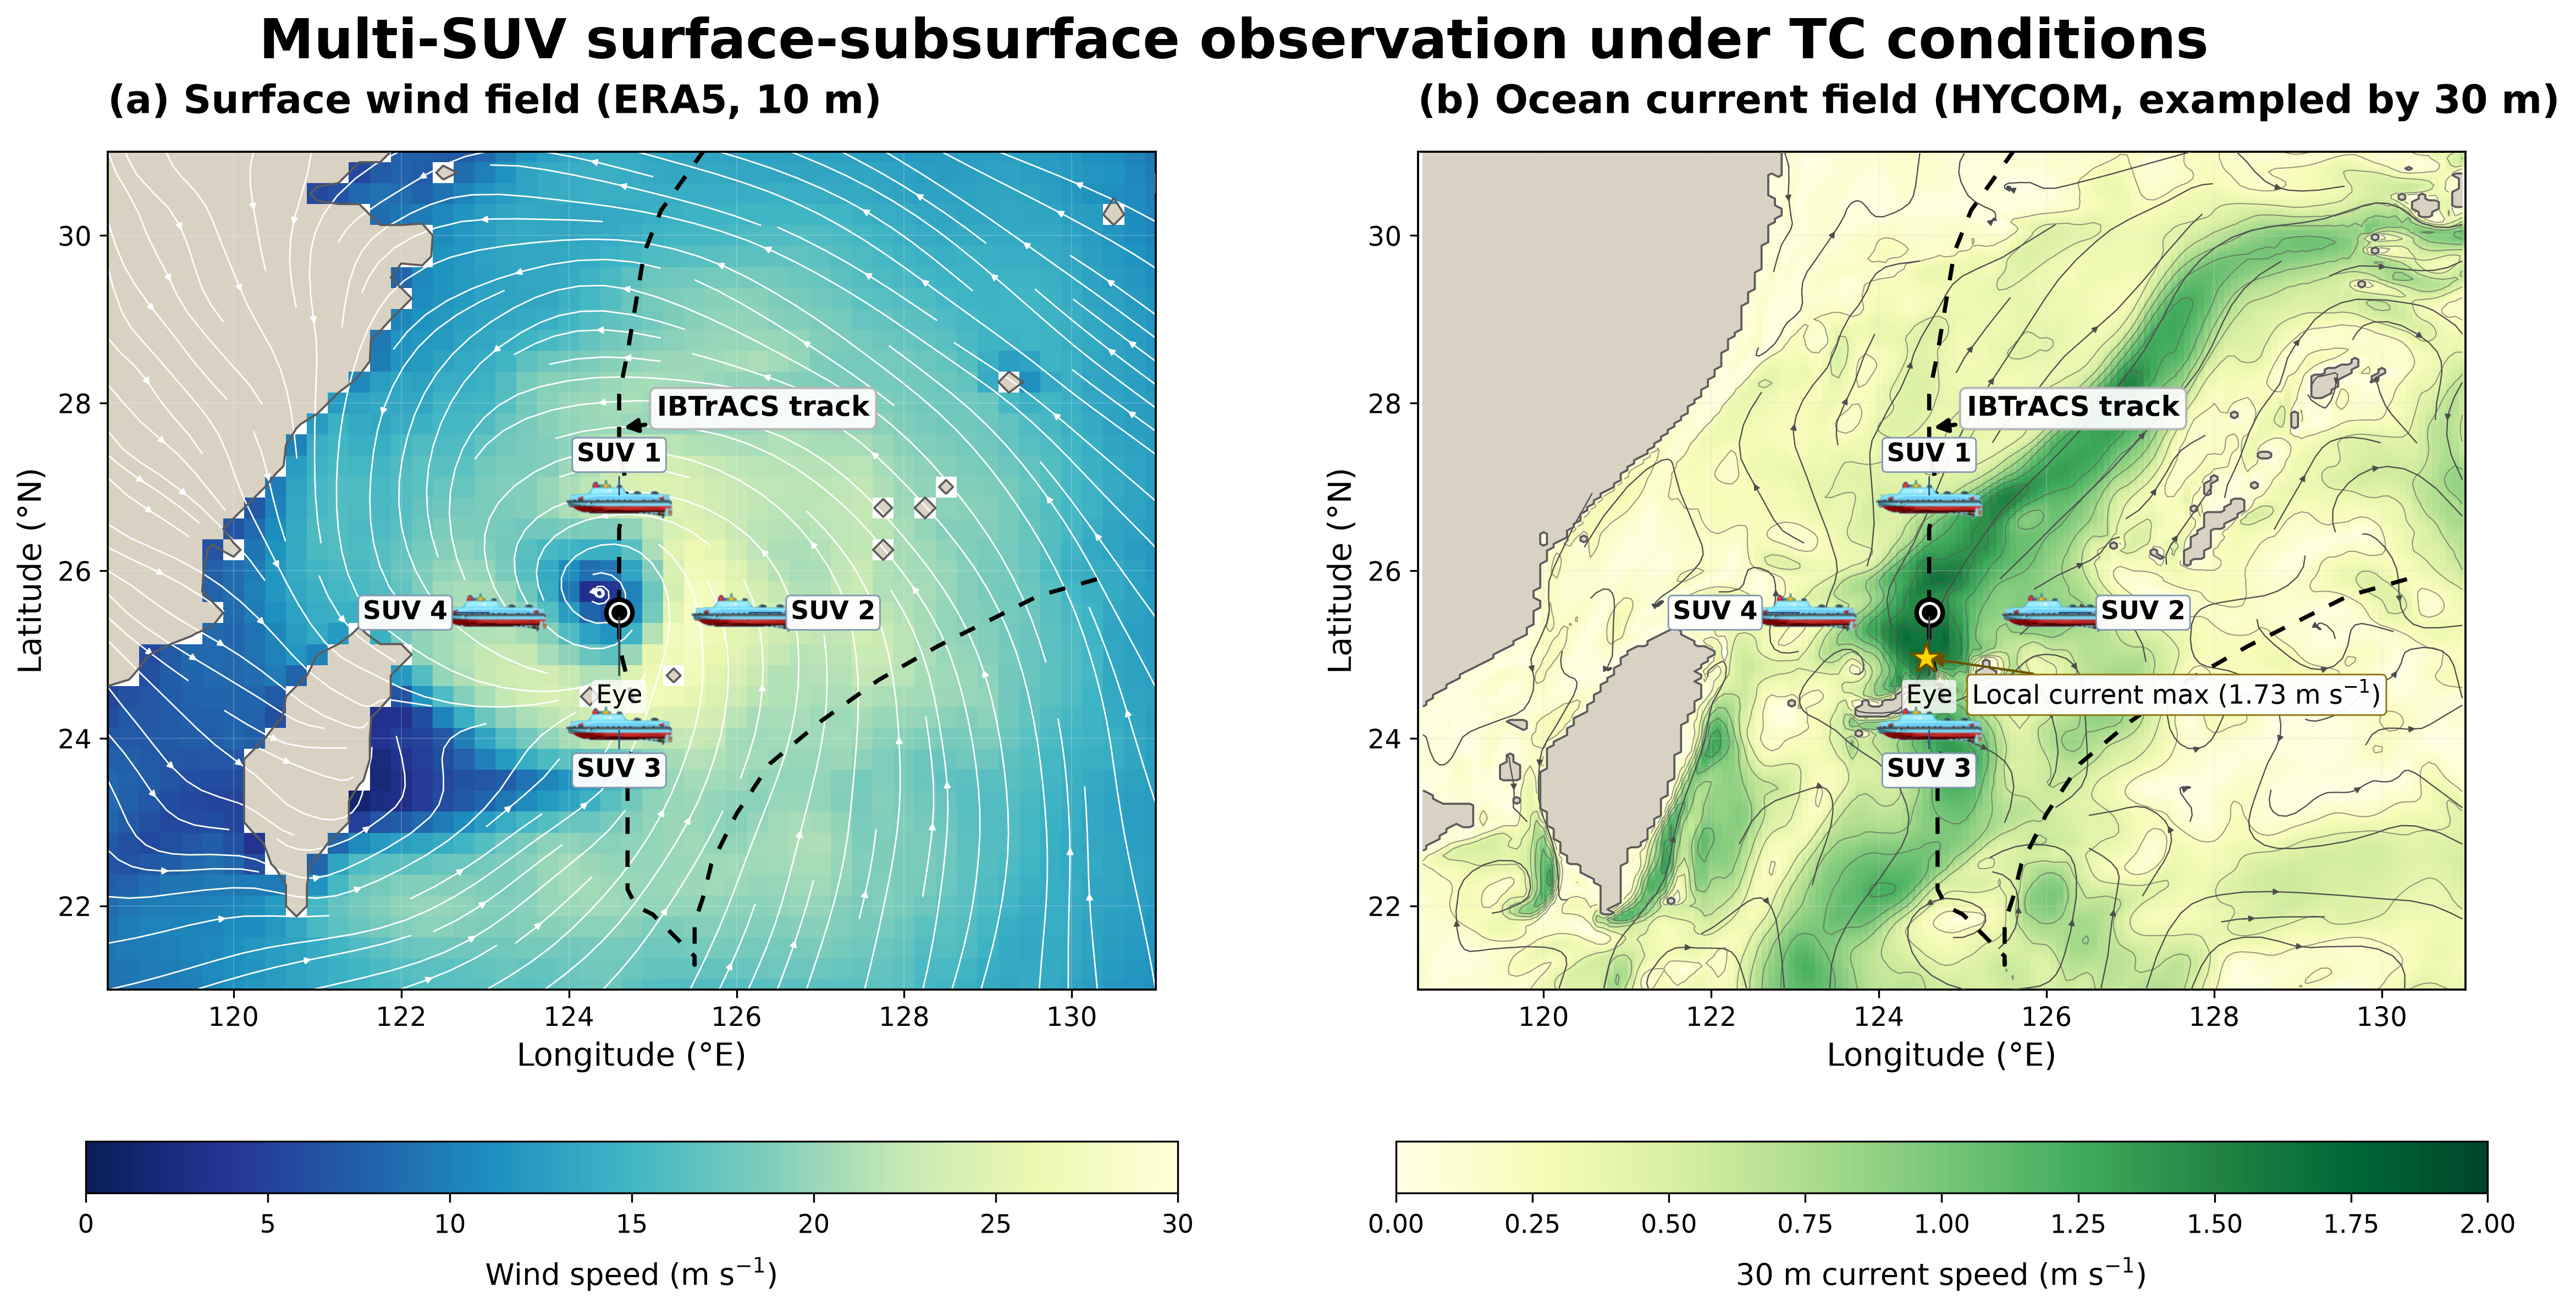
\includegraphics[width=\textwidth]
    {figures/Fig1_Surface_Subsurface_Observation.png}
\caption{Coordinated surface--subsurface TC observation for a representative
HINNAMNOR (2022) snapshot. The left panel shows four SUVs tracking the IBTrACS
best track while sampling ERA5 winds at 10 m above the sea surface. The right
panel shows the same formation sampling HYCOM currents at 30 m below the sea
surface; this depth is shown as an illustrative example, whereas the complete
experiments cover the seven depths from 0 to 60 m. The four-vehicle
configuration is illustrative, with equal angular spacing; subsequent
experiments evaluate fleets of 8, 12, and 16 vehicles.}
\label{fig:system_architecture}
\end{figure*}

Traditional graph search, sampling-based planning, potential fields, and model
predictive control are effective when the cost map and dynamics are known
\citep{r43,r44,r45,r46,r47,r48}. In a TC, however, the fields are nonstationary
and only locally observed, while propulsion is superimposed on ambient flow.
Conventional pipelines also estimate a field or waypoint sequence before
execution. By contrast, reinforcement learning (RL) maps each new measurement
directly to the next action, closing the observation--decision--motion loop.
RL has demonstrated strong sequential decision making across diverse domains
\citep{r49,r50,r51,r52,r53,r54,r55,r56}, and independent PPO is competitive in
cooperative multi-agent tasks \citep{r41,r42,r57}. Multi-AUV adaptive sampling
and target tracking provide the ocean-robotics foundations
\citep{r32,r33,r34,r35,r36}.

{\sloppy
Three gaps remain. First, a unified atmosphere--ocean reinforcement-learning
environment for coordinated surface--subsurface TC observation has not been
established \citep{r26,r27}. Second, it remains unclear whether
parameter-sharing MARL can track a moving TC under deployment uncertainty,
sample the subsurface current field, and remain effective across different
fleet sizes \citep{r23,r24,r25,r27}. Third, learned policies have rarely been
compared with causal planners under identical local observations, motion
constraints, and control interfaces. We formulate stochastic policy
optimization under partial observability \citep{r40,r41,r42}, evaluate 4-, 8-,
12-, and 16-SUV fleets, and provide this matched comparison.
\par}

The main contributions of this study are summarized as follows.
\begin{enumerate}
\item We construct a unified atmosphere--ocean RL environment by aligning ERA5
10 m winds, HYCOM currents at seven depths from 0 to 60 m, and IBTrACS tracks.
The final 400-TC dataset is divided at the TC level into 360 training TCs and
40 held-out evaluation TCs.
\item We evaluate an IPPO policy with globally shared surface-wind observations
and one joint formation action for 4-, 8-, 12-, and 16-SUV fleets. Subsurface
controllers retain decentralized current histories. Surface policies are tested at 100--800 km
deployment offsets, and subsurface policies are tested at seven depths and two
propulsion limits. Surface tracking statistics use episode medians, whereas
subsurface current and coverage statistics use episode means.
\item We compare IPPO with four traditional planners, including artificial
potential field, receding-horizon A*, lawnmower coverage, and
information-greedy control, under matched local observations, action
constraints, motion constraints, control intervals, and identical evaluation
episodes.
\end{enumerate}

\begin{figure*}[t]
\centering
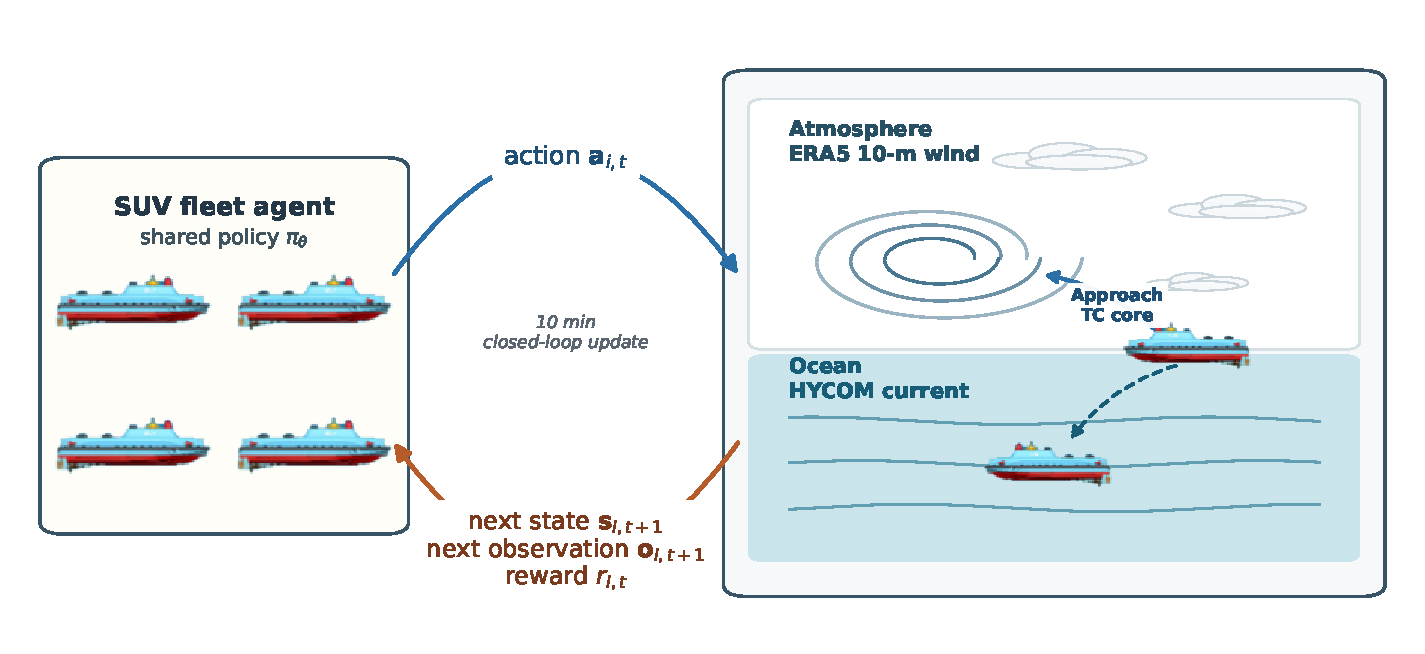
\includegraphics[width=\textwidth]
  {figures/Fig2_RL_Agent_Environment_Loop.pdf}
\caption{Closed-loop interaction between the SUV fleet agent and the
tropical-cyclone atmosphere--ocean environment. At each 10 min interval, the
SUV fleet agent perceives environmental information as observations. Its shared
policy $\pi_\theta$ maps the common surface observation to a joint formation
action. Underwater, each SUV maps its local current-history observation to an
independent action. The environment returns a reward and the next state to the
agent. In the
right panel, the rightmost surface SUV senses the local wind speed and moves
toward the TC core region. After reaching a more central position, represented
by the left surface SUV, the first-stage task is completed. The SUV then dives
vertically and begins the second-stage observation task at the prescribed depth,
collecting temperature, salinity, and current observations and intelligently
adjusting its motion based on the local current information.}
\label{fig:rl_loop}
\end{figure*}

\section{Problem Formulation}\label{sec:problem}

\subsection{Observation Task and Design Requirements}

The objective is to coordinate a fleet of submersible unmanned vessels
(SUVs) to observe a moving tropical cyclone (TC) across the sea surface and
upper ocean. At the surface, the SUV fleet navigates as a rigid formation toward
the moving TC core.
Final tracking error measures the fleet-center-to-TC-core distance remaining at
the end of the episode and serves as a proxy for access to the near-core high-wind regime. In the
operational concept, the fleet would descend after entering a predefined
terminal tracking region. The
learning experiments evaluate this mission as two separate episodes: a surface
approach episode and a subsurface sampling episode in which four SUVs seek the
highest attainable current speed at each prescribed depth. The mission imposes
four operational requirements:

\begin{enumerate}
\item rapid correction of initial deployment errors using surface propulsion;
\item tracking of the moving TC using onboard wind observations
and inter-vehicle observation sharing;
\item subsurface observation at ocean depths of 0, 10, 20, 30, 40, 50, and
60 m below the sea surface;
\item safe operation under action smoothing and coastline safeguards.
\end{enumerate}

The surface maximum speed is varied between 12 and 20 m/s, while the submerged
maximum propulsion speed is 1.5 or 2.0 m/s. This difference creates an
asymmetric decision problem: surface propulsion is used to follow the TC and
reduce the fleet-center-to-TC-core distance, quantified primarily by the final
tracking error. At the subsurface, the primary learning objective changes to
finding and sampling higher-current water, while geometric and current-weighted
spatial coverage characterize how broadly and how valuably the fleet samples
the dynamically active region. The four SUVs must balance active propulsion
against passive advection by the ambient current.

\subsection{Problem Definition}

The fleet contains $N$ SUVs, where $N\in\{4,8,12,16\}$, indexed by
$i\in\{1,2,\ldots,N\}$. The position, commanded horizontal velocity,
and operating mode of SUV $i$ at time $t$ are denoted by
$\mathbf{x}_i(t)$, $\mathbf{p}_i(t)$, and $m_i(t)\in\{\mathrm{s},\mathrm{u}\}$,
respectively, where $\mathrm{s}$ and $\mathrm{u}$ denote the surface and
subsurface modes. Horizontal positions and reported distances are expressed in
km, whereas commanded and ocean-current velocities are expressed in m/s. The
commanded speed satisfies
\begin{equation}
\|\mathbf{p}_i(t)\|\leq
\begin{cases}
V_{\max}^{\mathrm{s}}, & m_i(t)=\mathrm{s},\\
V_{\max}^{\mathrm{u}}, & m_i(t)=\mathrm{u}.
\end{cases}
\label{eq:speed_constraint}
\end{equation}

Each simulated episode is assigned to one stage, consistent with the separate
surface and subsurface environments used in training and evaluation. The mode
$m_i(t)$ selects the applicable speed bound and motion law for that episode;
continuous diving, ballast transitions, and resurfacing are not simulated
within a single decision trajectory.

For the motion equations, let \(\mathbf{p}_i\) denote the desired horizontal
velocity command and \(\mathbf{q}_i^{\mathrm{prop}}\) the effective propulsion
velocity after the acceleration and heading dynamics. The km/min
representation of the ocean current is denoted by
\(\mathbf{v}_{\mathrm{ocean}}\); the device-level speed bounds above remain
reported in m/s. The surface uses the effective propulsion velocity directly as
ground velocity, whereas the underwater stage adds current advection. The
horizontal motion in km is
\begin{equation}
\dot{\mathbf{x}}_i(t)=
\begin{cases}
\mathbf{q}_i^{\mathrm{prop}}(t), & m_i(t)=\mathrm{s},\\[1mm]
\mathbf{q}_i^{\mathrm{prop}}(t)+
\mathbf{v}_{\mathrm{ocean}}
\left(\mathbf{x}_i(t),z_i,t\right), & m_i(t)=\mathrm{u},
\end{cases}
\label{eq:platform_motion}
\end{equation}
where $z_i\in\{0,10,20,30,40,50,60\}$ m. Time $t$ is measured in minutes, and
$\mathbf{v}_{\mathrm{ocean}}(\cdot)$ is the HYCOM current at the corresponding
position and depth. Underwater ground velocity is the superposition of active
propulsion and background advection.

For numerical implementation, the continuous model is integrated explicitly at
the decision interval $\Delta t=10$ min:
\begin{equation}
\mathbf{x}_{i,k+1}=
\mathbf{x}_{i,k}+
\Delta t
\begin{cases}
\mathbf{q}_{i,k}^{\mathrm{prop}},
& m_{i,k}=\mathrm{s},\\[1mm]
\mathbf{q}_{i,k}^{\mathrm{prop}}+
\mathbf{v}_{\mathrm{ocean}}(\mathbf{x}_{i,k},z_i,t_k),
& m_{i,k}=\mathrm{u}.
\end{cases}
\label{eq:platform_motion_discrete}
\end{equation}
Here \(\Delta t=10\) min. The current field is evaluated at the beginning of
each interval and interpolated to the current vehicle position.
For the active underwater reward, we write this pre-move current as
$\mathbf{u}_{i,k}=\mathbf{u}_{\mathrm{ocean}}
(\mathbf{x}_{i,k},z_i,t_k)$.

To represent the dynamic constraints of the SUV, the desired command is
converted into a speed and course and then tracked under bounded acceleration,
deceleration, heading rate, and minimum turn radius. In the surface stage, the
command specifies a desired horizontal ground velocity, which is tracked
without an added current term. In the underwater stage, the command specifies a
desired propulsion velocity before current advection is applied:
\begin{equation}
\begin{aligned}
\mathbf{p}_{i,k}^{\mathrm{des}}
&=V_{\max}^{m_i}\tilde{\mathbf{a}}_{i,k},
\qquad
s_{i,k}^{\mathrm{des}}
=\left\|\mathbf{p}_{i,k}^{\mathrm{des}}\right\|_2,\\
\psi_{i,k}^{\mathrm{des}}
&=\operatorname{atan2}
\left(\bar a_{i,k,y},\bar a_{i,k,x}\right).
\end{aligned}
\label{eq:constrained_desired_speed_course}
\end{equation}
Each SUV carries an effective propulsion speed $s_i$ and heading $\psi_i$, with
$\mathbf{q}_i^{\mathrm{prop}}
=s_i[\cos\psi_i,\sin\psi_i]^{\top}$. The 10 min control interval is divided
into ten 60 s substeps. In substep $\ell$, speed and heading evolve according to
\begin{equation}
\begin{aligned}
s_i^{\ell+1}
&=\mathrm{clip}\!\left(
s_i^\ell\right.\\
&\quad\left.+
\mathrm{clip}\!\left(
s_{i}^{\mathrm{des}}-s_i^\ell,
-a_{m_i}^{\mathrm{dec}}\Delta\tau,
a_{m_i}^{\mathrm{acc}}\Delta\tau
\right),
0,V_{\max}^{m_i}
\right),\\
\bar\omega_i^{\ell+1}
&=\min\left(\omega_{\max}^{m_i},
\frac{s_i^{\ell+1}}{R_{\min}^{m_i}}\right),\\
\psi_i^{\ell+1}
&=\mathrm{wrap}\!\left[
\psi_i^\ell\right.\\
&\quad\left.+
\mathrm{clip}\!\left(
\mathrm{wrap}
\left(\psi_i^{\mathrm{des}}-\psi_i^\ell\right),
-\bar\omega_i^{\ell+1}\Delta\tau,
\bar\omega_i^{\ell+1}\Delta\tau
\right)
\right],
\end{aligned}
\label{eq:constrained_dynamics}
\end{equation}
where $\Delta\tau=60$ s. For the surface stage,
$a_{\mathrm{s}}^{\mathrm{acc}}=0.02$ m/s$^2$,
$a_{\mathrm{s}}^{\mathrm{dec}}=0.03$ m/s$^2$,
$\omega_{\max}^{\mathrm{s}}=1^\circ$/s, and
$R_{\min}^{\mathrm{s}}=200$ m. For the underwater stage,
$a_{\mathrm{u}}^{\mathrm{acc}}=0.002$ m/s$^2$,
$a_{\mathrm{u}}^{\mathrm{dec}}=0.003$ m/s$^2$,
$\omega_{\max}^{\mathrm{u}}=2^\circ$/s, and
$R_{\min}^{\mathrm{u}}=100$ m. The minimum-radius term is applied only while
the vehicle is moving; a commanded zero action decelerates the vehicle without
changing its course. The vehicle then advances over each substep using
\begin{equation}
\mathbf{x}\leftarrow\mathbf{x}+
\left(
\mathbf{q}_i^{\mathrm{prop}}+
\mathbf{1}_{\{m_i=\mathrm{u}\}}\mathbf{u}_{\mathrm{ocean}}
\right)\Delta\tau,
\label{eq:constrained_substep_translation}
\end{equation}
with the current held fixed over the 10 min control interval. Thus the surface
desired command is a ground velocity, whereas the underwater desired command is
a propulsion velocity before current advection. The speed is initialized to
zero and the heading is initialized uniformly in $[0,2\pi)$ at the beginning of
each episode.

The motion model remains a horizontal point mass model and does not
resolve added mass, hydrodynamic drag, roll and pitch, buoyancy and ballast
dynamics, thruster transients, wave loads, or actuator delay. ERA5 winds are
available at $0.25^\circ$ and hourly resolution, whereas HYCOM currents are
available at approximately $0.04^\circ$ by $0.08^\circ$ and three-hourly
resolution. These fields are interpolated to the 10 min decision interval and
to each vehicle position, but such interpolation does not recover
high-frequency wave forcing, local wake effects, or unobserved vehicle attitude
and actuator states. A detailed six-degree-of-freedom model would require
platform-specific hydrodynamic coefficients and forcing information that are
not commensurate with the present data, and could imply a level of numerical
precision unsupported by the inputs. The results therefore address planning and
coordination rather than structural loading or low-level controller response.

\subsection{Surface--Subsurface Two-Stage Task}
\label{subsec:handoff}

The SUVs first perform surface tracking, using coordinated propulsion to
follow the TC and reduce their distance to its center. For the operational protocol,
we assume that descent begins after the surface fleet enters the terminal
region defined by a final tracking error of at most 200 km. The simulation
uses this 200 km value as the upper bound on the tracking error at the
surface-to-subsurface transition and initializes the subsurface vehicles
within the corresponding 200 km disk around the TC core at the end time of
the surface segment. Because the present simulation does not model descent
dynamics, the surface and subsurface stages are represented as two
time-aligned but state-independent episodes. The descent duration is
simplified: after the surface stage, each vehicle is assumed to arrive
immediately at one prescribed depth. Each depth is a separate configuration
with four SUVs, and a single episode does not visit multiple depths.
At the end of the underwater observation task, the operational concept returns
the SUVs to the sea surface for recovery. This ascent and recovery phase is not
modeled here; the paper models only the surface observation-and-tracking stage
and the subsequent fixed-depth underwater observation stage.

The local observation of SUV $i$ is
\begin{equation}
\mathbf{o}_i(t)=
\begin{cases}
\left[\mathbf{s}_i(t),\,\mathbf{v}_i(t)\right],
& m_i(t)=\mathrm{s},\\[1mm]
\left[\mathbf{h}_i(t),\,\mathbf{v}_i(t)\right],
& m_i(t)=\mathrm{u},
\end{cases}
\label{eq:observation}
\end{equation}
where $\mathbf{s}_i(t)$ is the stage-specific measurement block,
$\mathbf{v}_i(t)$ is the normalized effective horizontal propulsion velocity
$\mathbf{v}_i=\mathbf{q}_i^{\mathrm{prop}}/V_{\max}^{m_i(t)}$, and
$\mathbf{h}_i(t)$ is an optional causal history block.
In the final surface experiments,
$\mathbf{s}_i(t)\in\mathbb{R}^{3N}$ contains the normalized speed and two wind
components at 10 m above the sea surface sampled by all $N$ SUVs; the surface
policy has no history block, and its effective ground velocity is augmented by
$[\cos\psi_i,\sin\psi_i]$.
Surface operation assumes idealized, lossless, and instantaneous
inter-vehicle communication: every SUV receives the wind observations acquired
by all other SUVs in the fleet as part of its policy input.
In the underwater IPPO evaluation, no inter-vehicle communication is
assumed. The observation contains no separate instantaneous-current block in
addition to the history; instead,
define the local current feature
$\mathbf{c}_{i,t}=[\|\mathbf{u}_{\mathrm{ocean}}(\mathbf{x}_{i,t},z_i,t)\|,
u_{\mathrm{ocean},x},u_{\mathrm{ocean},y}]^{\top}$, where
$\mathbf{u}_{\mathrm{ocean}}=(u_{\mathrm{ocean},x},
u_{\mathrm{ocean},y})$, and
$\mathbf{h}_i(t)=[\mathbf{c}_{i,t-4}^{\top},\ldots,
\mathbf{c}_{i,t}^{\top}]^{\top}\in\mathbb{R}^{15}$, which is the causal
five-frame history of SUV $i$'s current speed and two components at its
assigned depth; before five measurements are available, the earliest observed
frame is repeated to fill the history.
Each underwater SUV receives neither the current observations nor the positions
or actions of the other SUVs. The complete reanalysis field, the
global best-track center, and future environmental states are not provided to
the policy.
These two communication assumptions are intentionally different and mark the
bounds of the present study. The idealized global surface link represents a
favorable satellite or radio-connected operating mode, which makes it an
upper-bound assumption. The no-communication underwater case is the
conservative opposite bound: shared policy parameters are loaded separately on
each vehicle, but no observation, position, or action is exchanged at runtime.
The surface payload is one shared vector of $3N$ scalar wind values per fleet
decision, whereas the underwater inter-vehicle message payload is zero.
The reported experiments do not model bandwidth, packet loss, acoustic latency,
or intermittent surfacing. We do not present either the ideal surface link or
the fully decentralized subsurface case as a validated communication system.
The resulting surface observation dimension is
$d_o^{\mathrm{s}}=3N+4$. The underwater five-frame history contains
15 scalars; adding the two normalized propulsion components and
the heading representation $[\cos\psi_i,\sin\psi_i]$ gives
$d_o^{\mathrm{u}}=19$.

During training, the reward function can access the distance between each SUV
and the best-track TC core. This distance supervises the association between
local 10 m wind patterns and proximity to the TC core/high-wind region; the
center coordinate itself is not an actor input. During validation, rewards do
not influence actions. The trained policy receives only the shared fleet-level
wind samples and must track an unseen TC, thereby testing whether the learned
wind-to-center relation generalizes.

The normalized action is
\begin{equation}
\mathbf{a}_i(t)\in[-1,1]^2,
\end{equation}
and is projected onto the unit disk before being mapped to a desired velocity
command in both modes:
\begin{equation}
\tilde{\mathbf{a}}_i(t)=
\frac{\mathbf{a}_i(t)}
{\max\left(1,\|\mathbf{a}_i(t)\|_2\right)},\qquad
\mathbf{p}_i(t)=
V_{\max}^{m_i(t)}\tilde{\mathbf{a}}_i(t).
\label{eq:normalized_action}
\end{equation}
For the surface task, the hard formation constraint is imposed by sharing both
the observation and the action:
\begin{equation}
\mathbf{o}_{i,t}=\mathbf{o}_t,\qquad
\mathbf{a}_{i,t}=\mathbf{a}_t,
\qquad i=1,\ldots,N.
\label{eq:rigid_formation_action}
\end{equation}
The formation center is
$\bar{\mathbf{x}}_{e,t}=N^{-1}\sum_i\mathbf{x}_{i,e,t}$, and the initial
relative offsets
$\mathbf{r}_i=\mathbf{x}_{i,e,0}-\bar{\mathbf{x}}_{e,0}$ are held constant.
Because the surface model excludes water currents and all SUVs receive the same
dynamic command, each vehicle undergoes the same translation while preserving
its initial ring, line, grid, or V-shaped geometry. For the subsurface task,
the action remains vehicle-specific because each SUV observes only its own
current history.
This mapping ensures that the desired and effective speeds never exceed the
mode-specific speed limit. Here \(\bar{\mathbf{a}}_i(t)\) is the executed
normalized command after action smoothing, unit-disk projection, and any
stage-specific safety projection; without a safety intervention,
\(\bar{\mathbf{a}}_i(t)=\tilde{\mathbf{a}}_i(t)\).
In the surface stage, the action specifies a desired ground velocity. In the
underwater stage, the same unit-disk command specifies a desired propulsion
speed and course. In both stages, the effective speed and heading evolve
according to the dynamics defined above.

\subsection{Cooperative Action Formulation}\label{subsec:decpomdp}

The cooperative task uses a shared-action partially observable Markov decision
process at the surface and a decentralized partially observable Markov decision
process (Dec-POMDP) at the subsurface:
\begin{equation}
\mathcal{M}=
\left\langle
\mathcal{I},
\mathcal{S},
\{\mathcal{A}_i\},
P,
R,
\{\Omega_i\},
O,
\gamma
\right\rangle,
\label{eq:decpomdp}
\end{equation}
where $\mathcal{I}$ is the set of SUVs, $\mathcal{S}$ is the joint environment
state, $\mathcal{A}_i$ and $\Omega_i$ are the local action and observation
spaces of vehicle $i$,
$P(s_{t+1}\mid s_t,\mathbf{a}_t)$ is the transition probability,
$R(s_t,\mathbf{a}_t,s_{t+1})\in\mathbb{R}^{N}$ is the local-reward vector, and
$O(\mathbf{o}_{t+1}\mid s_{t+1},\mathbf{a}_t)$ is the joint observation
function. The shared team reward before clipping is
$\bar r_t=N^{-1}\sum_{i=1}^{N}r_{i,t}$, where
$r_{i,t}$ is the $i$th element of
$R(s_t,\mathbf{a}_t,s_{t+1})$, and $\gamma$ is the discount factor.
For the surface stage, $\mathcal{A}_i=\mathcal{A}$ and
$\Omega_i=\Omega$ for every SUV, and the joint action is constrained to
$\mathbf{a}_{1,t}=\cdots=\mathbf{a}_{N,t}=\mathbf{a}_t$. The resulting process
is a centralized partially observable control problem for the rigid formation.
For the subsurface stage, the action and observation spaces remain
vehicle-specific as in a conventional Dec-POMDP.

At each 10 min interval, the policy forms a closed
perception--decision--action loop and does not follow a precomputed route:
\begin{equation}
\begin{aligned}
\text{surface: }&
\mathbf{o}_{t}\rightarrow
\mathbf{a}_{t}=\pi_\theta(\mathbf{o}_{t})
\rightarrow
\{\mathbf{x}_{i,t+1}\}_{i=1}^{N}
\rightarrow
\mathbf{o}_{t+1},\\
\text{subsurface: }&
\mathbf{o}_{i,t}\rightarrow
\mathbf{a}_{i,t}=\pi_\theta(\mathbf{o}_{i,t})
\rightarrow
\mathbf{x}_{i,t+1}
\rightarrow
\mathbf{o}_{i,t+1}.
\end{aligned}
\label{eq:closed_loop}
\end{equation}
The updated observation becomes the next control input. This feedback structure
lets the fleet adapt to changing wind and current fields,
partial observability, and deployment uncertainty without a static waypoint
sequence. Fig.~\ref{fig:rl_loop} summarizes this interaction between the moving
atmosphere--ocean environment and the cooperative SUV fleet.

\section{Data and Simulation Environment}\label{sec:data}

\subsection{Reanalysis and Best-Track Products}

ERA5 supplies hourly zonal and meridional wind components at 10 m above the sea
surface on a regular $0.25^\circ$ grid
\footnote{ERA5 download portal:
\url{https://cds.climate.copernicus.eu/datasets/reanalysis-era5-single-levels}.}
\citep{r37}. Wind speed and direction are calculated from
$u_{10}$ and $v_{10}$. HYCOM supplies three-hourly zonal and meridional
currents at ocean depths of 0, 10, 20, 30, 40, 50, and 60 m below the sea
surface
\footnote{HYCOM GLBy0.08 dataset:
\url{https://www.hycom.org/data/glby0p08/expt-93pt0}; HYCOM ESPC-D-V02 dataset:
\url{https://www.hycom.org/data/espcd-v02}.}
\citep{r38}. The native horizontal grid is
approximately $0.04^\circ$ in latitude by $0.08^\circ$ in longitude. IBTrACS
provides TC time, center position, maximum wind, minimum pressure, and related
metadata at mostly 3 or 6 h intervals
\footnote{IBTrACS download portal:
\url{https://www.ncei.noaa.gov/products/international-best-track-archive}.}
\citep{r39}. The dataset-selection domain used to identify candidate systems is
$98.7^\circ$E--$171.6^\circ$E and $6.8^\circ$N--$56.7^\circ$N. The TC events
span October 2007 to December 2025 UTC. The surface observation
variable is the 10 m wind speed and
direction, whereas the subsurface observation variables are the horizontal
current velocity, represented by \texttt{water\_u} and \texttt{water\_v}, and
the derived current speed over the 0--60 m layer.
Table~\ref{tab:data} summarizes the products, variables, native grids, and
temporal resolutions used to construct the simulation environments.

\begin{table*}[htbp]
\centering
\caption{Environmental datasets used to construct the 400-TC observation
environments. The dataset integrates ERA5 surface winds, HYCOM currents at
seven depths, and IBTrACS best tracks.}
\label{tab:data}
\resizebox{\textwidth}{!}{%
\begin{tabular}{@{}lllll@{}}
\toprule
Data product & Source & Variables used & Native grid & Native time \\
\midrule
Surface wind at 10 m above sea level & ERA5 & $u_{10}$, $v_{10}$, speed, direction &
$0.25^\circ \times 0.25^\circ$ & Hourly \\

Current at 0--60 m ocean depth & HYCOM & \texttt{water\_u}, \texttt{water\_v},
speed at 0/10/20/30/40/50/60 m &
$\sim0.04^\circ$ lat $\times 0.08^\circ$ lon & 3-hourly \\

Best track & IBTrACS & Position, time, wind, pressure & Point track &
Mainly 3/6-hourly \\
\bottomrule
\end{tabular}}
\par\smallskip
\parbox{\textwidth}{\footnotesize
Note: although the SUV platform can carry sensors for observing temperature,
salinity, and currents, the reinforcement-learning policy uses only surface
wind and subsurface current observations as environmental inputs.}
\end{table*}

\subsection{Spatiotemporal Alignment and Track Segmentation}

Hourly ERA5 winds and three-hourly HYCOM currents are linearly interpolated to
a common 10 min simulation clock and queried at each SUV position. The
environmental trajectories are precomputed and do not respond to vehicle
motion; this one-way forcing assumption is appropriate for planning at the
scale of a TC. The policy receives only local reconstructed
values at the current time, not future fields or the complete reanalysis map.
The best-track center is used only for training rewards and evaluation.

Commands are held constant within each decision interval:
\begin{equation}
\mathbf{a}_i(t)=\mathbf{a}_{i,k},
\quad t_k\leq t<t_{k+1},
\quad t_{k+1}-t_k=\Delta t=10\ \mathrm{min}.
\label{eq:zero_order_hold}
\end{equation}
The environmental fields, TC track, action, and position update use the same
time grid. The 10 min step balances control responsiveness against
the hourly and three-hourly resolution of the source products; a shorter step
would add samples without adding resolved information. The same interval is
used for IPPO and all traditional planners.

Each IBTrACS track is first linearly interpolated to the 10 min simulation
interval. The cumulative along-track distance is computed using the local
equirectangular approximation
\begin{equation}
\Delta s_k =
\sqrt{
\left[
111\Delta\lambda_k\cos(\varphi_k)
\right]^2
+
\left(111\Delta\varphi_k\right)^2
},
\label{eq:segment_distance}
\end{equation}
where $\Delta\lambda_k$ and $\Delta\varphi_k$ are longitudinal and latitudinal
increments in degrees, and 111 km is the mean meridional arc length per degree.
Target segment lengths are sampled uniformly from 300--500 km, with a fixed
250 km stride, 50--250 km overlap, and an average overlap of about 150 km.
Residual track shorter than 300 km is discarded. After assignment to 10 min
track samples, the final realized lengths range from 292.1 to 505.5 km, with a
median of 396.1 km.

The IBTrACS archive contains 540 tropical cyclones in the study domain between
October 2007 and December 2025 UTC. We retain TCs with aligned ERA5 and HYCOM
products and apply two data-quality screens. First, for each candidate segment,
every 10 min TC position must remain at least 200 km from land. Second, we
remove segments that start at the TC formation boundary (\(t_0=0\)) and
segments that extend beyond the final valid IBTrACS timestamp; the latter
prevents constant-position extrapolation at the end of a track. The resulting
400-TC dataset contains 3,392 segments. The 360 training TCs contribute 3,130
segments, whereas the 40 held-out TCs contribute 262 segments. The split is made
at the TC level, so no TC appears in both sets. Segment durations range from 2.2
to 97.5 h. The median duration was 15.3 h and the mean was 17.7 h. These segments provide mission-scale
evaluation windows. The platform can carry
current, CTD, pH,
chlorophyll, and turbidity sensors \citep{r28}, while the control experiments
use current velocity as the decision-making observation.

\section{Multi-Agent Reinforcement Learning Method}\label{sec:model}

\subsection{Blue Whale-Class Platform Modeling}

Each SUV is represented by a horizontal point mass model with mode-dependent speed
bounds and position updates from
Eqs.~\eqref{eq:speed_constraint}--\eqref{eq:platform_motion}. The surface actor
uses globally shared 10 m wind observations and outputs one common velocity
command for the rigid formation, whereas the underwater actor uses a causal
five-frame history of its local current and normalized velocity. The surface control variable is defined in the
Earth-fixed frame as a desired ground velocity. Therefore, ocean-current
compensation is not included as a separate term in the surface position update.
Underwater motion retains advection because 1.5--2.0 m/s propulsion is
comparable to the TC-induced current.

The two simulation configurations compare present and potential future
platform capabilities. The 12 m/s surface and 1.5 m/s submerged limits are
close to the public Blue Whale design speeds, whereas 20 m/s and 2.0 m/s
represent a future-upgrade case. Table~\ref{tab:platform} reports the complete
parameterization and distinguishes modeling assumptions from certified
specifications.

\begin{table*}[htbp]
\centering
\caption{Public Blue Whale reference and the two simulation configurations.
The second simulation column is a simple parameterization of the present-day
reference platform, whereas the third represents a possible future-upgrade
configuration with higher surface and subsurface speeds for comparison. These
scenarios are modeling assumptions, not certified vehicle data.}
\label{tab:platform}
\resizebox{\textwidth}{!}{%
\begin{tabular}{@{}p{0.22\textwidth}p{0.22\textwidth}p{0.22\textwidth}p{0.22\textwidth}@{}}
\toprule
Property & Public reference & Current-platform scenario & Future-upgrade scenario \\
\midrule
Surface speed & 23 kn, $\approx$11.83 m/s &
12 m/s & 20 m/s \\

Submerged speed & 3 kn, $\approx$1.54 m/s &
1.5 m/s & 2.0 m/s \\

Public-reference submerged endurance &
$\geq$4 h at 3 kn; $\geq$72 h standby & -- & -- \\

Underwater evaluation horizon & -- &
20 h simulation & 20 h simulation \\

Sampling depth & $\approx$60 m & 0--60 m, seven layers &
0--60 m, seven layers \\

Payload & $\geq$800 kg & 800 kg & 800 kg \\

Surface fleet size & Single platform & 4/8/12/16 & 4/8/12/16 \\

Decision interval & Not specified & 10 min & 10 min \\

Surface formation & -- & 100 km ring, $360^\circ/N$ &
100 km ring, $360^\circ/N$ \\
\bottomrule
\end{tabular}}
\end{table*}

Across 28,506 IBTrACS track samples, the median, 95th-percentile, and
99th-percentile TC translation speeds are 5.14, 13.89, and 20.58 m/s
(Table~\ref{tab:tc_speed_envelope}). The 12 and 20 m/s surface limits cover
93.0\% and 98.8\% of these samples, respectively. The submerged limits cover
only 3.3\% and 7.0\% of the samples. For the subsurface task, the SUVs are
initialized randomly within a 200 km radius of the TC core and perform local
adaptive sampling; the task does not attempt to overtake or continuously follow
the moving TC core.

\subsection{Parameter-Sharing Independent PPO}
\label{subsec:ippo}

All SUVs contribute to the same tracking objective, and the training return is
defined as the team-average reward. At the surface, the cooperative task is
represented by a single joint formation action for the whole fleet. At the
subsurface, each SUV retains an independent action and local observation.

For the surface task, IPPO optimizes one two-dimensional joint formation action
from the shared fleet observation, and every SUV executes this same action.
The fixed relative offsets in Eq.~\eqref{eq:rigid_formation_action} constitute
a hard constraint rather than a reward penalty. For the subsurface task, IPPO
uses parameter sharing with vehicle-specific observations and action samples.
The main surface model uses a memoryless multilayer perceptron, whereas the
active underwater controller uses a five-frame current history. The shared
cooperative return is the team-average reward. The surface value estimate is
\(V_\phi(\mathbf{o}_t)=v_\phi(\mathbf{o}_t)\), whereas the subsurface estimate
sums the local values, \(V_\phi(\mathbf{o}_t)=\sum_{i\in\mathcal{I}}
v_\phi(\mathbf{o}_{i,t})\). A single clipped PPO objective is optimized over
the surface formation action or the factorized multi-agent subsurface action:
\begin{equation}
\begin{aligned}
L^{\mathrm{CLIP}}(\theta)
={}&\mathbb{E}_t\Bigl[
\min\Bigl(
\rho_t(\theta)\hat A_t,\\
&\qquad
\operatorname{clip}
\left(\rho_t(\theta),1-\epsilon,1+\epsilon\right)
\hat A_t
\Bigr)\Bigr],
\end{aligned}
\label{eq:ppo}
\end{equation}
where
\begin{equation}
\rho_t(\theta)=
\prod_{i\in\mathcal{I}}
\frac{\pi_\theta(a_{i,t}\mid o_{i,t})}
{\pi_{\theta_{\mathrm{old}}}(a_{i,t}\mid o_{i,t})},
\label{eq:ratio}
\end{equation}
and $\hat A_t$ is estimated by generalized advantage estimation from the
team-average reward. The actor objective is complemented by a clipped value
loss and an entropy bonus. For the surface stage, the product in
Eq.~\eqref{eq:ratio} reduces to the single shared-action likelihood. For the
subsurface stage, it retains the vehicle-specific likelihoods. During surface
execution, one policy query produces $\mathbf{a}_t$, which is transmitted
unchanged to every SUV. Underwater, each SUV computes its own action from its
local observation and the shared policy network. The complete training and
deployment procedure is summarized in Algorithm~\ref{alg:ippo_training}.

\begin{algorithm*}[t]
\caption{Training and deployment of shared-action surface IPPO and independent subsurface IPPO}
\label{alg:ippo_training}
\begin{algorithmic}[1]
\REQUIRE Training TC split, stage-specific environment, fleet size $N$,
speed limit $V_{\max}$, reward coefficients, and random seed
\ENSURE Shared actor and critic parameters
\STATE Initialize the actor, critic, and parallel environment workers
\FOR{training iteration $m=1,\ldots,M$}
  \STATE Reset the stage-specific environment and obtain the common surface
  observation $\mathbf{o}_t$, or the local observations
  $\mathbf{o}_{i,t}$ for all $i=1,\ldots,N$ underwater
  \FOR{rollout step $t$}
    \IF{surface stage}
      \STATE Sample or select one joint formation action
      $\mathbf{a}_t\sim\pi_\theta(\cdot\mid\mathbf{o}_t)$ as the joint
      formation action for all SUVs
    \ELSE
      \STATE Sample or select a local action for each SUV from
      $\pi_\theta(\cdot\mid\mathbf{o}_{i,t})$
    \ENDIF
    \STATE Apply the stage-specific action filter, unit-disk projection, and
    common formation safety filtering
    \STATE Advance all SUVs and collect the team-average reward
  \ENDFOR
  \STATE Compute GAE advantages and returns for the team-average reward
  \STATE Update the shared actor and critic with the clipped PPO objective
\ENDFOR
\STATE Freeze the actor and load the same parameters on every SUV
\FOR{each deployment episode}
  \STATE Observe local or shared data according to the stage communication model
  \STATE Compute the shared surface action, or the local subsurface action,
  from the policy
  \STATE Apply action smoothing, circular projection, and safety filtering
  \STATE Execute the action and observe the next state
\ENDFOR
\end{algorithmic}
\end{algorithm*}

To compare reinforcement-learning algorithm choices, IPPO, SAC, and TD3 were
trained for the same \(2\times10^6\) environment steps on representative
surface and subsurface cases with two independent training seeds. Surface
metrics are summarized by episode medians and underwater metrics by episode
means before averaging across the two seeds. This comparison is used only as
bounded algorithm-choice evidence. IPPO requires no replay buffer and is
therefore used for the main, formation, and planner comparisons.

The complete reward coefficients, safety parameters, network dimensions, and
PPO hyperparameters are summarized in Appendix~\ref{app:parameters}.

\subsection{Surface and Subsurface Reward Design}

The surface objective is to follow the translating TC as closely as possible
and reach the high-wind region, with the final tracking error as the
primary operational metric. Let $d_{i,k+1}$ denote the post-transition
distance from SUV $i$ to the TC core after executing the command at decision
step $k$, and let $\bar{\mathbf{a}}_{i,k}$ denote the executed command after
filtering and unit-disk projection. The surface reward used in the
implementation is
\begin{equation}
\begin{aligned}
r_i^{\mathrm{surf}}={}&
-\frac{\min(d_{i,k+1},D_{\max})}{D_{\mathrm{scale}}}
+b_{\mathrm{near}}\mathbf{1}_{d_{i,k+1}<d_{\mathrm{near}}}\\
&-\frac{W_{\mathrm{form}}
\max(0,d_{i,k+1}-R_{\mathrm{form}})}{D_{\mathrm{scale}}}\\
&-\lambda_u\|\bar{\mathbf{a}}_{i,k}
-\bar{\mathbf{a}}_{i,k-1}\|_2^2
+r_i^{\mathrm{coast}},
\end{aligned}
\label{eq:surface_reward}
\end{equation}
where the first term is a bounded proximity cost and the second term provides
a discrete near-center bonus with $b_{\mathrm{near}}=1$. Here
\(D_{\max}=300\) km caps the proximity cost, \(D_{\mathrm{scale}}=100\) km
normalizes the distance terms, and \(d_{\mathrm{near}}=100\) km defines the
near-center reward region. The third term adds an additional radius-excess
penalty beyond $R_{\mathrm{form}}=100$ km, and the fourth term penalizes abrupt
action changes with $\lambda_u=0.05$. The term $r_i^{\mathrm{coast}}$
represents the coastal-safety reward defined below. The 300 km cap prevents
distant errors from producing an excessively steep gradient and reduces
premature policy collapse during early training. After aggregation over SUVs,
the team average reward is clipped to $[-5,2]$.

For subsurface observation, four SUVs are assigned to each prescribed depth.
Their primary objective is not to follow the surface TC core directly, but to
observe the highest possible current speed. Geometric and current-weighted
spatial coverage are then evaluated as complementary measures of observation
extent and observation value. Low-speed SUVs cannot generally overtake a
translating TC, and the vertical projection of the surface center is not
necessarily the location of the strongest subsurface current. For subsurface
IPPO training, the current-seeking reward is
\begin{equation}
\begin{aligned}
r_i^{\mathrm{sub}}={}&
\min\left(
\frac{\|\mathbf{u}_{i,k}\|}{V_{\mathrm{norm}}},
R_{\max}
\right)\\
&-\lambda_a\|\tilde{\mathbf{a}}_{i,k}\|_2^2
+\beta_{\parallel}\max(0,\cos\theta_i)\\
&+r_i^{\mathrm{coast}},
\end{aligned}
\label{eq:sub_reward}
\end{equation}
where $V_{\mathrm{norm}}=1.0$ m/s, $R_{\max}=2.0$,
$\lambda_a=0.05$, and $\beta_{\parallel}=0.5$. The term
$-\lambda_a\|\tilde{\mathbf{a}}_{i,k}\|_2^2$ penalizes large normalized
propulsion commands and regularizes the action magnitude. The angle $\theta_i$
denotes the direction difference between the effective propulsion velocity and
the pre-move current
$\mathbf{u}_{i,k}$, so the positive-alignment term is activated only when the
SUV pushes downstream; formally, we define \(\cos\theta_i=0\) when either
vector is zero and otherwise set
$\cos\theta_i=
(\mathbf{q}_{i,k}^{\mathrm{prop}}\cdot\mathbf{u}_{i,k})/
(\|\mathbf{q}_{i,k}^{\mathrm{prop}}\|_2\|\mathbf{u}_{i,k}\|_2)$.
The current-intensity reward is evaluated at $\mathbf{x}_{i,k}$ before the
state update.

\subsection{Coastal Safety and Action Smoothing}

The land mask is converted into a nonnegative offshore-distance field. A vehicle
inside land receives a large penalty, and a vehicle within the buffer distance
$D_{\mathrm{buf}}$ receives
\begin{equation}
r_i^{\mathrm{coast}}=
\begin{cases}
-P_{\mathrm{land}}, & D_i=0,\\
-W_b\max(0,1-D_i/D_{\mathrm{buf}}), & 0<D_i<D_{\mathrm{buf}},\\
0, & D_i\geq D_{\mathrm{buf}},
\end{cases}
\label{eq:coast}
\end{equation}
where $D_i=D(\mathbf{x}_{i,k+1})$ is the post-transition offshore distance,
with $D_i=0$ on land, and $P_{\mathrm{land}}$ and $W_b$ are positive penalty
coefficients.

For the surface stage, three complementary mechanisms reduce coastline
intrusion: offshore-only rejection sampling during deployment, a soft nearshore
penalty, and an action-level safety filter. The main surface experiments use a
minimum deployment distance of 100 km, a 100 km nearshore buffer, and a 100 km
safety margin. Best-of-rejection deployment favors offshore initial states, the
reward discourages trajectories near land, and the safety filter removes the
onshore action component when an SUV approaches the shoreline. For the
subsurface stage, the nearshore penalty is retained and an episode is truncated
at landfall, but offshore-only initialization and action-level safety filtering
are not applied.

To reduce control oscillations and thereby lower mean speed and shorten path
length, the main surface experiments use an exponential action filter:
\begin{equation}
\mathbf{a}^{\mathrm{filt}}_k=
(1-\beta)\mathbf{a}^{\mathrm{raw}}_k+
\beta\mathbf{a}^{\mathrm{filt}}_{k-1},
\label{eq:filter}
\end{equation}
where $\beta\in[0,1)$ controls the degree of temporal smoothing. The filter
uses only the current and previous actions, which prevents future-information
leakage. The filtered command
$\mathbf{a}^{\mathrm{filt}}_k$ is then passed through the unit-disk projection
and speed mapping in Eq.~\eqref{eq:normalized_action}.

\subsection{Surface and Subsurface Evaluation}
\label{subsec:evaluation}

The center-distance reward is used only during training and is absent from
validation. Validation tests whether a trained policy can infer the TC direction
from wind observations in unseen events. The primary surface metric is the
final tracking error, defined for each validation episode as the
fleet-center-to-TC-core distance at the final time step. A smaller value places
the fleet closer to the TC core, where near-core winds are generally stronger.
The mean tracking error is the episode-level time average of the
fleet-center-to-TC-core distance and is reported as a secondary process
diagnostic. For both indicators, the reported validation statistic is the
median across validation episodes rather than the arithmetic mean.
Subsurface metrics instead use the arithmetic mean over validation episodes
within each trained policy seed; the reported uncertainty is the sample
standard deviation of those seed-level means.

For episode \(e\) at decision step \(k\), the formation center is
\begin{equation}
\bar{\mathbf{x}}_{e,k}
=
\frac{1}{N}\sum_{i=1}^{N}\mathbf{x}_{i,e,k}.
\label{eq:surface_formation_center}
\end{equation}
For episode \(e\), the episode-level mean tracking error is
\begin{equation}
d_{e}^{\mathrm{avg}}
=
\frac{1}{K_e}
\sum_{k=1}^{K_e}
\left\|
\bar{\mathbf{x}}_{e,k}
-
\mathbf{x}_{\mathrm{TC},e,k}
\right\|_2,
\label{eq:episode_time_average_distance}
\end{equation}
where \(K_e\) is the number of post-transition decision intervals. For training
seed \(s\), the reported final and mean tracking errors are the medians over
validation episodes:
\begin{equation}
D_{\mathrm{final}}^{(s)}
=
\operatorname*{median}_{e=1,\ldots,M_s}
\left\|
\bar{\mathbf{x}}_{e}(T_e)
-
\mathbf{x}_{\mathrm{TC},e}(T_e)
\right\|_2,
\label{eq:final_tracking_error}
\end{equation}
\begin{equation}
D_{\mathrm{mean}}^{(s)}
=
\operatorname*{median}_{e=1,\ldots,M_s}
d_{e}^{\mathrm{avg}},
\label{eq:time_averaged_distance}
\end{equation}
where \(T_e\) is the final decision time of validation episode \(e\), \(M_s\)
is the number of validation episodes, and distance is computed from the
formation center rather than from each SUV independently. The reported value
is the arithmetic mean of the seed-level medians.
The traditional planners are deterministic and have no training seed. Their
reported statistics are therefore medians over all paired validation
episodes; different deployment realizations are treated as validation
episodes, not as trained-model seeds.

The median is used because episode-level tracking errors are strongly
right-skewed. A small number of episodes can produce terminal errors far above
the typical case, particularly when another active TC produces a competing
wind signature or when the local wind field provides a weak and unstable
centre-directed gradient. An arithmetic mean would let these rare cases
dominate the reported central tendency even though they do not represent
nominal operation. These cases remain in the evaluation and are discussed
explicitly in Section~\ref{subsec:surface_results} and in the limitations,
rather than being silently removed from the evaluation set.

Surface evaluation covers 4/8/12/16 SUVs on a 100 km ring with equal angular
spacing. The formation-center offset represents the random position error of a
TC track forecast: it is equivalent to deploying the fleet at the corresponding
distance from the true TC core with a randomly selected bearing, after which
the SUVs move toward the TC. During training, formation-center offsets are
sampled uniformly within an 800 km radius, covering deployment-error scenarios
from 0 to 800 km. During evaluation, the trained policies are tested at fixed
radii of 100, 200, 400, 600, and 800 km to quantify how the magnitude of the
forecast-induced deployment error affects tracking performance. Metrics are
first summarized by the median over validation episodes within each seed and
then averaged across independent training seeds.

For the subsurface evaluation, each depth from 0, 10, 20, 30, 40, 50, and
60 m is tested as a separate 20 h configuration with four SUVs and 1.5 or
2.0 m/s speed limits. We assume that, after tracking under the 0--800 km random
surface deployment errors, the fleet reaches a core region within 200 km of the
TC core and begins descent. Underwater performance is evaluated under this
condition. Because descent time and vehicle-by-vehicle endpoint transfer are
not modeled, each SUV is initialized directly at its assigned depth, with the
formation center sampled uniformly within a 0--200 km radius of the TC core.
Thus, 200 km represents the current upper bound of the residual random position
error of the formation center relative to the TC core at the
surface-to-subsurface transition, rather than a fixed operating limit. As SUV
performance improves, this core-region threshold could be tightened to 100 or
50 km; the present experiments use 200 km. There is no inter-vehicle
communication, so each SUV uses only its own five-frame current history and
propulsion state.
IPPO and the traditional planners are evaluated on the same episodes,
deployment seeds, motion model, and speed bound. The IPPO policy uses its
deterministic mean action during evaluation.

For underwater evaluation, we consider three metrics: mean experienced current
speed, geometric coverage, and current-weighted coverage. The first metric
measures the current intensity encountered along each SUV's trajectory. Let
\(K\) be the number of recorded position increments, let \(k=0,\ldots,K\)
index the archived positions, and let \(z\) denote the observation depth. The
time-averaged experienced current speed of SUV \(i\) in episode \(e\) is
\begin{equation}
\bar V_{i,e}(z)=\frac{1}{K_e+1}\sum_{k=0}^{K_e}
\left\|\mathbf{u}_{\mathrm{ocean}}
(\mathbf{x}_{i,k},z,t_k)\right\|_2.
\label{eq:experienced_current}
\end{equation}
where only valid ocean positions are included; a terminal on-land position is
excluded from the current and coverage statistics.
The reported fleet value is the average
\(N^{-1}\sum_{i=1}^{N}\bar V_{i,e}(z)\). A higher value indicates that the SUVs
spent more of their trajectories in stronger-current regions, but this metric
does not quantify how broadly the fleet sampled the surrounding area.

Geometric coverage measures the unique ocean area sampled by the fleet in
episode \(e\):
\begin{equation}
C_e(z)=A_{\mathrm{cell}}
\left|
\bigcup_{i=1}^{N}\bigcup_{k=0}^{K_e}
\mathcal{G}(\mathbf{x}_{i,k})
\right|,
\label{eq:underwater_coverage}
\end{equation}
where \(\mathcal{G}(\mathbf{x})\) is the \(0.25^\circ\) grid cell containing
position \(\mathbf{x}\), using the lower-left corner of the aligned event
domain as the grid origin; \(|\cdot|\) counts unique cells, and
\(A_{\mathrm{cell}}\approx(0.25^\circ\times111\ \mathrm{km})^2\approx770.06\
\mathrm{km}^2\) is the nominal grid-cell area used for cross-method comparison.
A larger \(C_e(z)\) indicates a
broader spatial sampling footprint, while repeatedly visiting the same cell
does not increase this metric. Coverage alone, however, does not distinguish
whether the sampled cells contain strong or weak currents.

To represent both current intensity and spatial extent, we define the
episode-level current-weighted coverage
\begin{equation}
\mathcal{C}_{\mathrm{w},e}(z)=
\left[
\frac{1}{N}\sum_{i=1}^{N}\bar V_{i,e}(z)
\right]C_e(z),
\label{eq:current_weighted_coverage}
\end{equation}
and aggregate it by taking the arithmetic mean over validation episodes within
each training seed, followed by the mean and sample standard deviation of the
seed-level means. This quantity assigns a higher value when strong-current
observations are combined with a broad sampling footprint. It therefore
captures observation value more directly than either the mean experienced
current or geometric coverage alone.

For all three underwater metrics, values are first averaged over the validation
episodes within each training seed and then averaged across the ten independent
seeds.
\subsection{Traditional Planning Baselines}\label{subsec:classical_planning}

To provide a non-learned reference for the learned cooperative policy, we next
introduce four traditional planning baselines.
We include four non-learned planners as secondary references
\citep{r44,r46,r48}. The artificial-potential-field planner moves along the
local gradient of observed wind or current speed and adds an offshore
repulsion inside the coastal buffer. The receding-horizon A* planner builds an
online local value map, re-plans a three-step minimum-cost route, executes the
first action, and refreshes the plan every 15 decisions. The boustrophedon
lawnmower planner follows fixed parallel coverage legs with phase offsets
between vehicles and uses no environmental value map. The information-greedy
planner evaluates eight candidate unit actions and selects the one with the
largest predicted local wind or current value plus the coastal preference.

None of the planners receives the TC core, the complete reanalysis field,
future frames, or the learned policy state. Surface planners use the same
shared wind samples and fleet navigation state as IPPO. Underwater, each
vehicle maintains a private map because communication is disabled. All four
use the same 10 min interval, speed envelope, circular projection, surface
safety filter. They require no training and have no training-seed variance.
Surface planners are evaluated
on all 262 held-out segments. Underwater planners use identical sets of 400
evaluation episodes per depth-speed setting. These episodes comprise 40 test
TCs with ten deployment seeds each.

\section{Simulation and Results}

\subsection{Surface Active Tracking}\label{subsec:surface_results}

Using the evaluation protocol in Section~\ref{subsec:evaluation}, we evaluate
the trained surface policies across four fleet sizes, two speed limits, five
deployment radii, and ten independent training seeds. Final tracking error
in Eq.~\eqref{eq:final_tracking_error} is the primary metric. Mean tracking error
is a secondary diagnostic of how closely the fleet remains to the
moving TC, while path length and mean ground speed characterize motion demand.

\begin{figure*}[t]
\centering
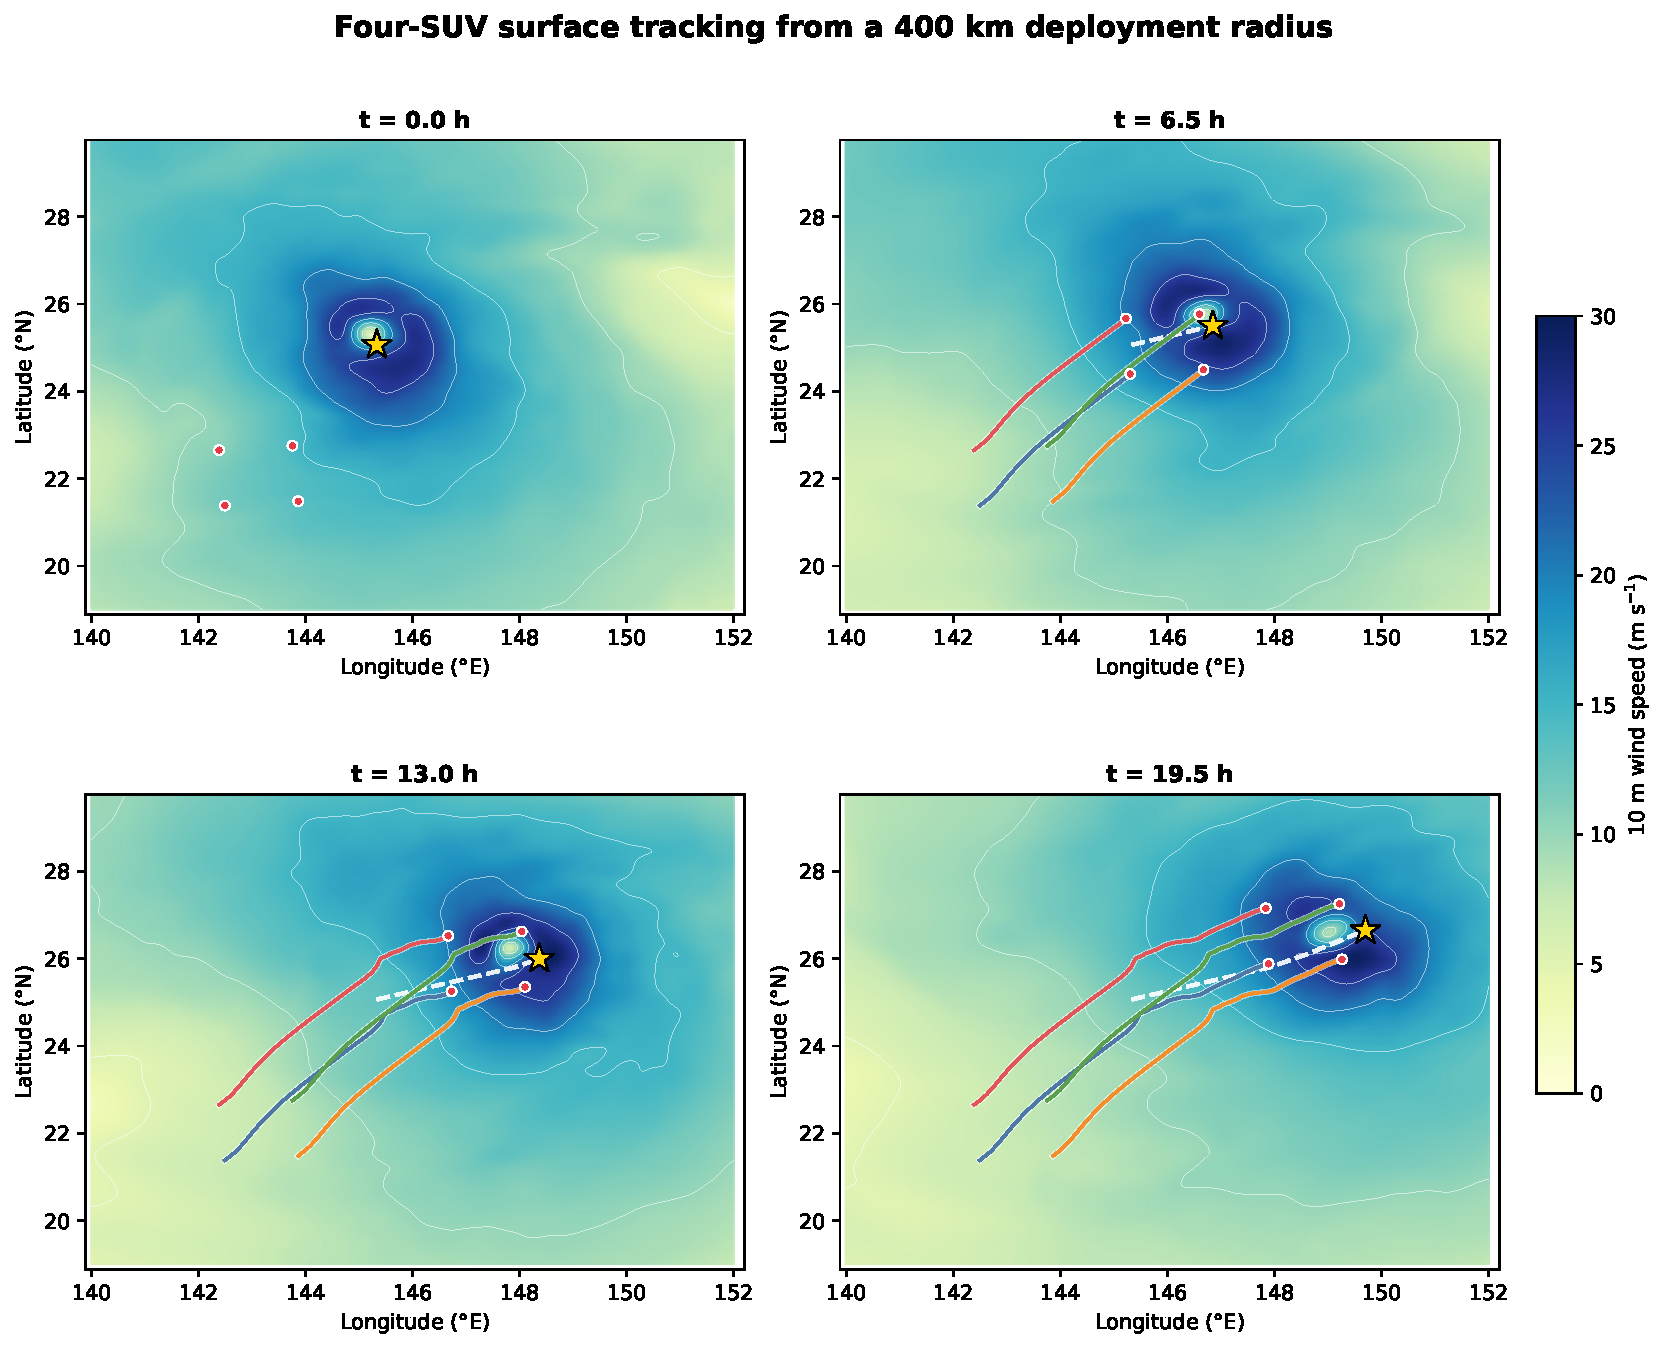
\includegraphics[width=\textwidth]
  {figures/Fig2_Surface_Trajectory_Evolution.pdf}
\caption{Four-SUV surface-tracking process for KHANUN (2023) at the 20 m/s
speed limit. The four panels show the initial deployment and subsequent
states at approximately 6.5, 13.0, and 19.5 h. The color background is the
spatially interpolated ERA5 10 m wind-speed field at each time. The formation
center is deployed at a fixed distance of 400 km from the TC core using a
randomly selected bearing. The fleet continually adjusts its trajectory toward
the TC core, and the displayed fleet-center-to-TC-core distance decreases
from 400.0 km at deployment to 44.8 km at the end of the episode. Small red
dots mark vehicle positions, and the yellow star marks the TC core.}
\label{fig:surface_trajectory_evolution}
\end{figure*}

\begin{figure*}[t]
\centering
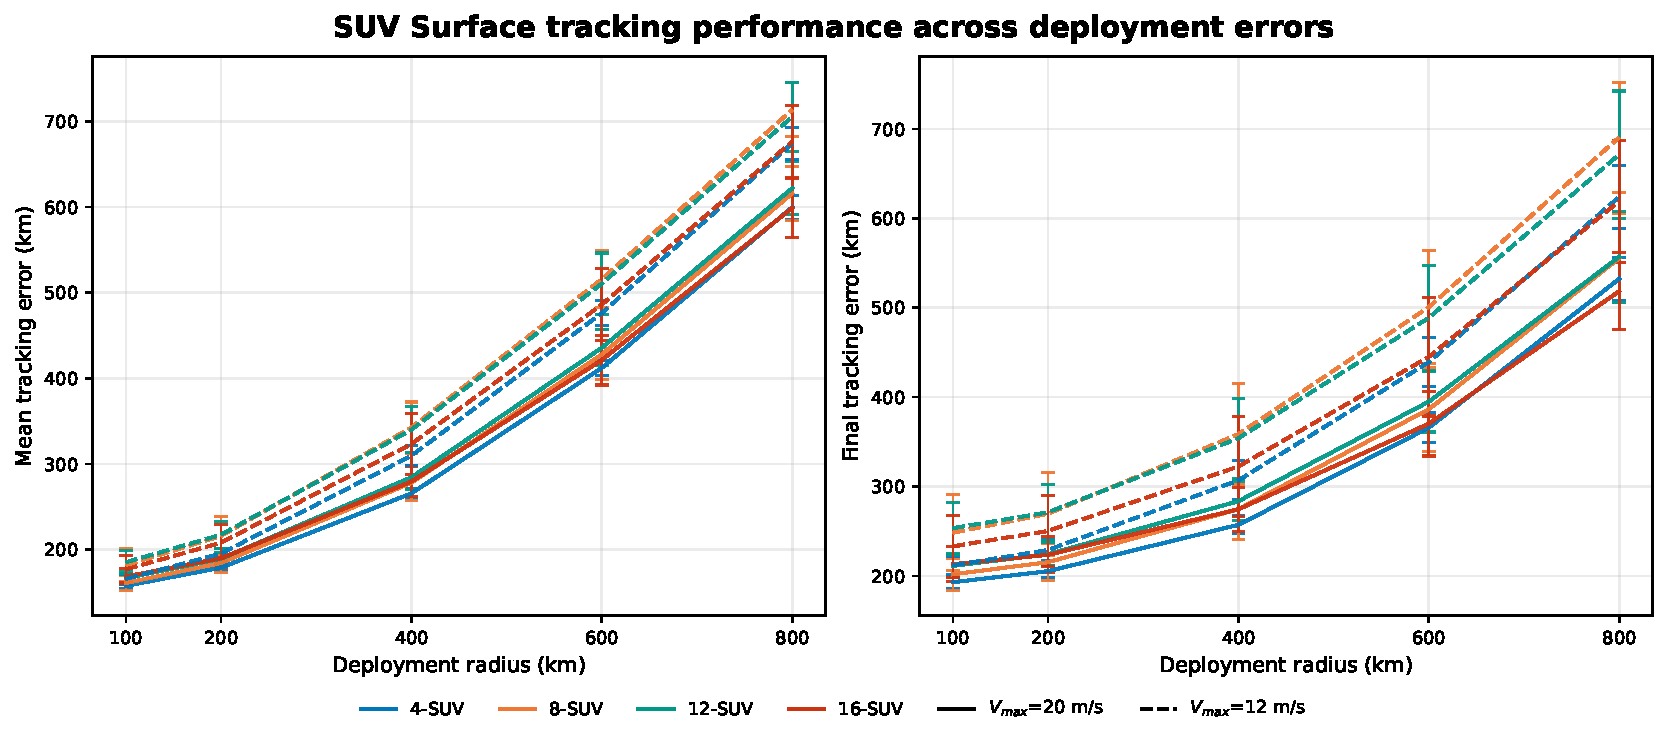
\includegraphics[width=\textwidth]
  {figures/Fig3_Surface_Vmax_Distance_Comparison.pdf}
\caption{SUV surface tracking performance across deployment errors. The left panel
shows the mean tracking error, defined as the mean fleet-center-to-TC-core
distance throughout an episode. The right panel shows the final tracking error,
defined as the fleet-center-to-TC-core distance at the end of the episode;
smaller values indicate a closer fleet center to the TC core. Colors denote
fleet sizes and line styles denote the 20 and 12 m/s speed limits. Each point
summarizes ten independent training runs using ten random seeds. Error bars
show the sample standard deviation.}
\label{fig:surface_vmax_comparison}
\end{figure*}

Figure~\ref{fig:surface_vmax_comparison} reports the population-level
speed-limit comparison. Averaged over fleet sizes and training seeds, the
20 m/s policy obtains final tracking errors of 204.8, 217.2, 272.5, 379.3, and 540.8 km
at deployment radii of 100, 200, 400, 600, and 800 km. The corresponding
12 m/s values are 236.7, 255.1, 335.5, 468.4, and 651.3 km. Thus, 20 m/s gives
the lower final tracking error in all 20 matched fleet-size/radius comparisons, and its
fleet-averaged advantage grows from 31.9 km at 100 km to 110.5 km at 800 km.
Both policies remain farther from the center as deployment error increases,
because finite speed and episode duration cannot remove every initial
displacement.

The mean tracking error shows the same ordering: 20 m/s has the smaller
distance in all 20 matched comparisons, with a median 12-minus-20 m/s difference
of 49.7 km on identical evaluation episodes. The two-sided tests on identical
evaluation episodes give $p<0.05$ in every case; these tests are exploratory
because they are not corrected across the 20 comparisons. The final-tracking-error
benefit is larger than the mean-tracking-error benefit at both ends of the
deployment range, indicating that the higher-speed policy
continues reducing residual separation late in the episode.

The 12 m/s policy reduces path length per SUV by 83.4--220.1 km across the five
radii and lowers mean ground speed by 1.75--3.93 m/s, whereas the 20 m/s policy
achieves closer final tracking.

The representative trajectories clarify how the aggregate result is produced.
Fig.~\ref{fig:surface_trajectory_evolution} follows the four-SUV, 400 km
KHANUN case. The vehicles first turn along the observed wind structure and then
reduce their separation from the center; by 19.5 h they have entered the
high-wind branch. The hard formation constraint keeps the relative offsets fixed, so the
individual paths are parallel translations of the same formation trajectory.

Figure~\ref{fig:surface_trajectory_matrix} separates the effects of fleet size
and deployment error. At 100--200 km, the formations converge rapidly and stay
concentrated near the TC core. At 600--800 km, trajectories lengthen and fan
out before turning inward, and final positions remain farther from the center.
Increasing the fleet from 4 to 16 SUVs adds sample branches and broadens the
approach region, but it does not replace the long-range transit. In the
representative 12- and 16-SUV cases, paths overlap near the TC core once the
shared wind observations guide the fleet toward the same high-wind region.
Deployment error therefore controls the required transit distance, whereas
fleet size mainly controls how broadly the approach is sampled.

Two retained long-tail episodes illustrate why the median is preferred for the
main statistics. The first is the 2012 MARIA--PRAPIROON dual-TC case. Although
MARIA is the designated target, PRAPIROON is simultaneously present in the
same ERA5 wind field. The competing TC produces a stronger and more coherent
local wind signature along part of the route, and the shared-observation policy
moves into the corresponding branch, ending farther from the designated MARIA
centre. This
case reflects ambiguity in a multi-TC environment rather than the nominal
single-target behaviour. The second is a 2021 OMAIS episode at a 200 km
deployment radius. Around the fleet centre, the mean local wind speed is only
about 4.2 m/s and the mean horizontal wind-speed gradient is approximately
\(0.008\ \mathrm{m\,s^{-1}\,km^{-1}}\). Such a weak gradient does not provide a
persistent centre-directed signal, so the policy can maintain an incorrect
heading for a prolonged period. These episodes are retained in the evaluation
and are revisited as limitations below; because they occupy the far tail, the
median better represents typical performance than the arithmetic mean.

\subsection{Surface Formation Comparison}
\label{subsec:formation_comparison}

The ring, line, grid, and V-shaped formations provide four different ways to
allocate spatial observations across eight SUVs. The V formation places four
SUVs symmetrically on each arm. To make the comparison independent of total
formation size, all four layouts are normalized to the same mean radius of
100 km. This common mean radius keeps the fleet spatially spread out and allows
it to acquire broader and more numerous coverage observations. This experiment
is a matched single-seed sensitivity study: all four policies use training seed
0, the same 2-million-step protocol, deployment distribution, and safety layer
at both 12 and 20 m/s, and are evaluated without retraining at 100--800 km
(Table~\ref{tab:formation_comparison}). Averaged over the ten speed--radius
conditions, the line gives the lowest mean final tracking error of 320.8 km, followed by
the V formation at 323.1 km, the ring at 341.2 km, and the grid at 396.0 km.
The line is best in six speed--radius conditions, and the V formation is best
in the remaining four conditions at 100--600 km under 12 m/s. The ring is best
at 800 km under 12 m/s. The V formation also lowers the mean tracking error to
330.8 km, compared with 332.5 km for the line, 348.4 km for the ring, and
377.4 km for the grid.

The mean radius is 100 km for every formation. It is a prescribed geometric
property of the initial layout and does not change during an episode under the
hard formation constraint.

The grid produces the shortest per-vehicle path, averaging 392.7 km, followed
by the ring at 416.5 km, the line at 482.6 km, and the V formation at 499.8 km.
The path differences show that the initial arrangement changes the transit
effort even though each formation remains rigid after deployment.

Figure~\ref{fig:formation_comparison} visualizes one matched KHANUN segment.
Each policy issues one joint formation action, so the initial geometry is preserved
throughout the episode. This representative episode visualizes how the same
joint formation action produces different spatial trajectories from the four
initial arrangements. Because the deployment bearing relative to the TC core is
random, the policy cannot assume that the cyclone lies in a fixed direction.
The ring formation uses \(360^\circ/N\) equal angular spacing and provides
direction-independent, approximately isotropic spatial sampling around the
formation center. At the same mean radius, the line and V formations concentrate
observations along limited directions, whereas the grid concentrates them at a
discrete set of locations, especially its corners. We therefore use the ring as
the robust default for the main experiments, without claiming that it is
optimal for every tracking or path metric. The line, V, and grid formations are
reported as sensitivity cases and reflect different emphasis on tracking error
and path length. Because only training seed 0 is used, these formation-specific
differences are not interpreted as statistically resolved population effects;
the ten-seed analysis is reserved for the main ring configuration.

\begin{figure*}[p]
\centering
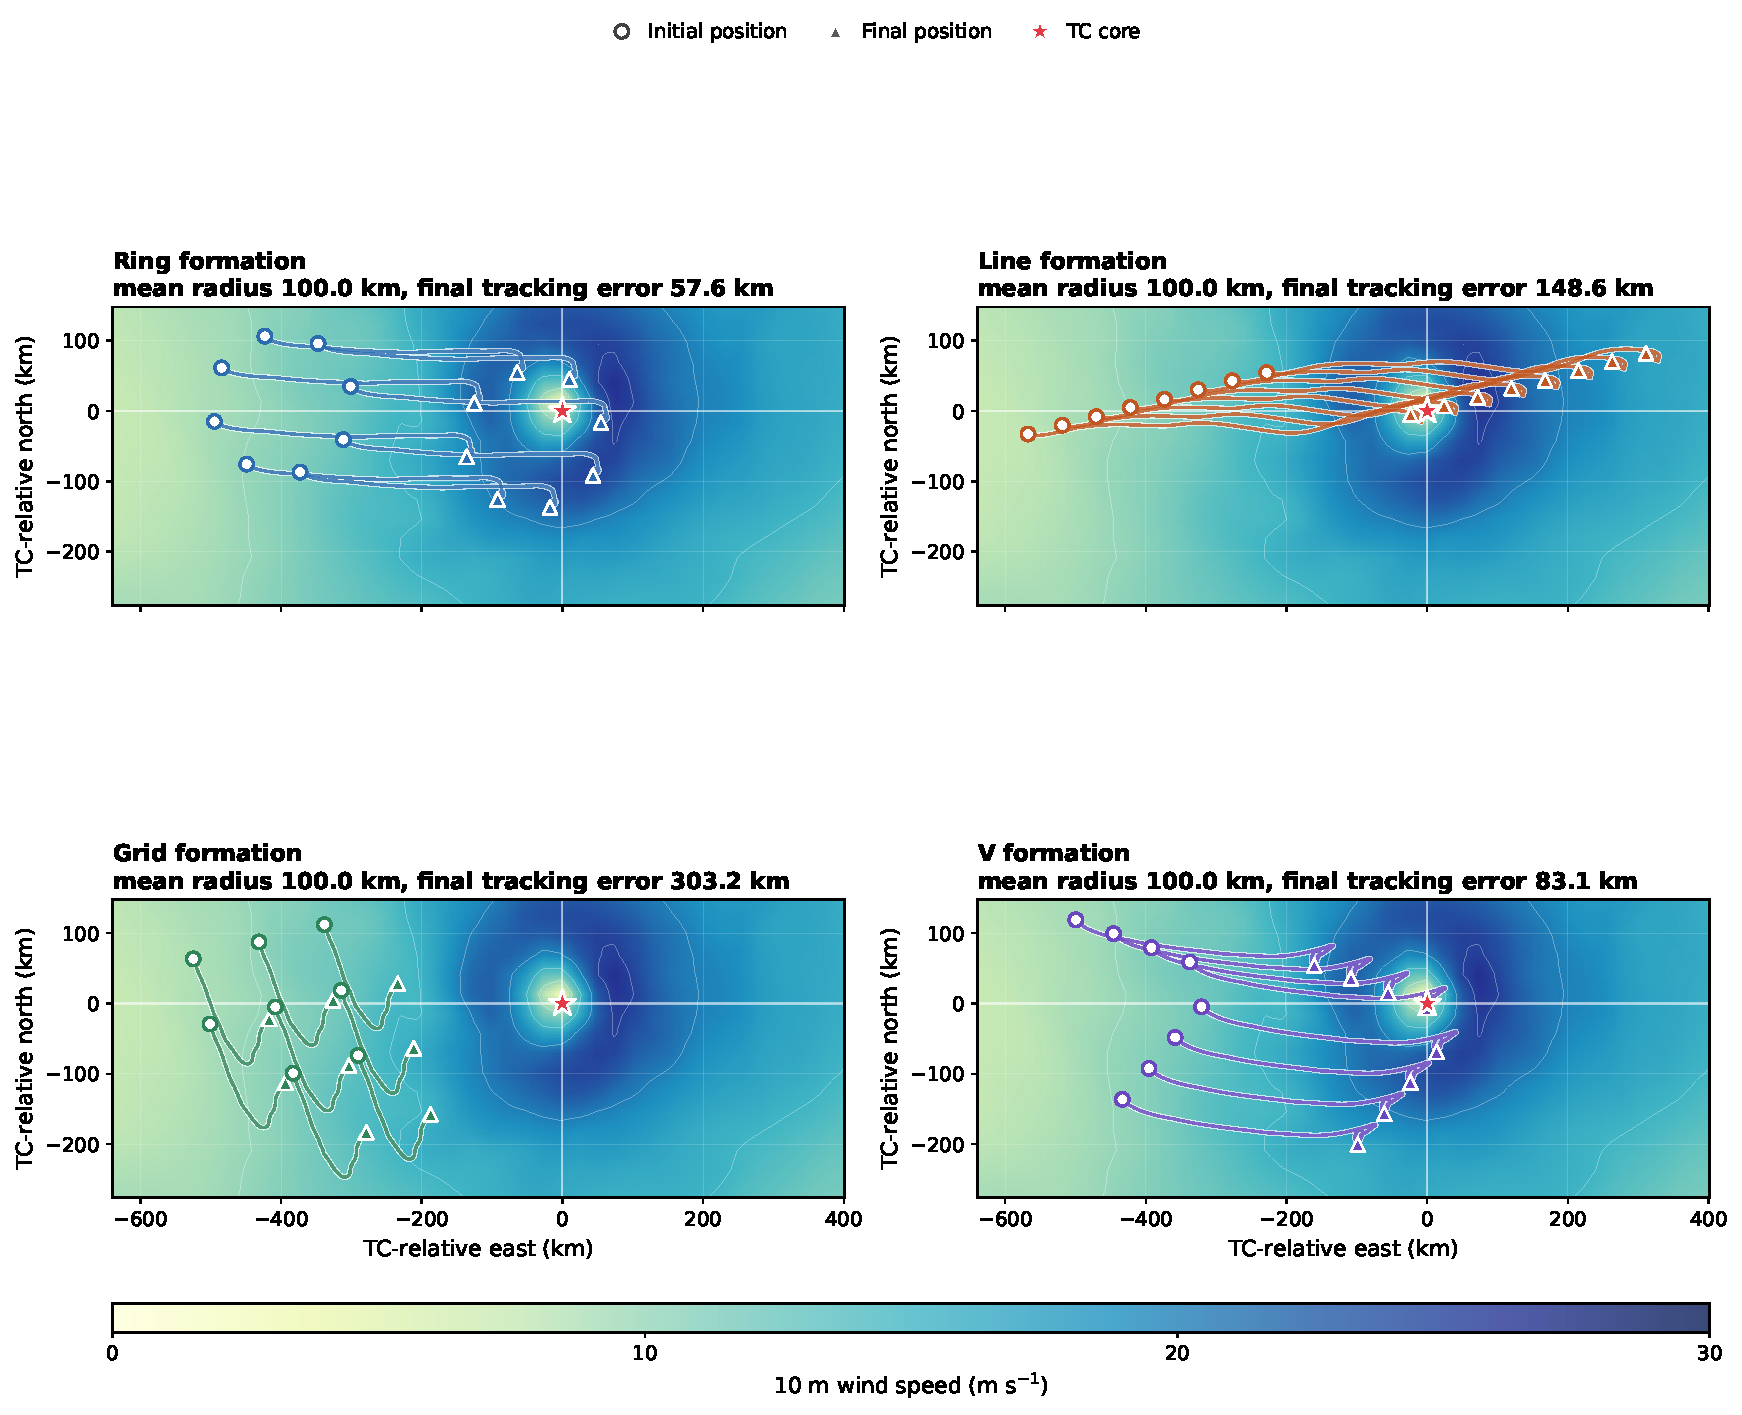
\includegraphics[width=\textwidth]{figures/FigB1_Formation_Comparison.pdf}
\caption{Representative surface trajectory comparison for ring, line, grid,
and V-shaped formations with eight SUVs at 12 m/s. All layouts use the same
mean radius of 100 km. The formation center is deployed at a distance of 400 km
from the TC core using a randomly
selected bearing. Open circles denote initial positions,
triangles denote final positions, and the red star denotes the TC core. The
color background and contours show the spatially interpolated ERA5 10 m
wind-speed field at the final simulation step. Axes are relative to the
instantaneous TC core.}
\label{fig:formation_comparison}
\end{figure*}

\subsection{Execution-Layer Action Filtering}
\label{subsec:filtering}

In preliminary rollouts, the unfiltered commands changed direction
frequently, causing the SUVs to turn repeatedly and accumulate avoidable path
length and propulsion changes. Fig.~\ref{fig:filter_path_comparison} illustrates
this behavior: the unfiltered trajectories form
sawtooth-like detours, whereas filtering produces smoother paths under the same
policy and initial positions. We therefore added an execution-layer low-pass
filter that smooths successive commands while preserving the 10 min decision
interval. Table~\ref{tab:surface_control_ablations} quantifies this change
using the same trained actors over identical validation episodes. Without
filtering, the 4-, 8-, 12-, and 16-SUV
configurations travel 1019.2--1160.0 km per vehicle, with mean speeds of
14.85--16.45 m/s and maximum speeds of 19.46--19.47 m/s. With the
execution-layer filter ($\beta=0.8$), path length falls to 497.4--670.8 km,
mean speed to 8.49--11.01 m/s, and maximum speed to 14.25--17.97 m/s.
The final tracking error changes from 355.4 to 251.3 km for four SUVs, from
324.7 to 277.8 km for eight SUVs, from 312.0 to 278.8 km for 12 SUVs, and from
260.2 to 256.1 km for 16 SUVs. Averaged over the four fleet sizes, it decreases
from 313.1 to 266.0 km, a reduction of 47.1 km or 15.0\%. Filtering improves
final tracking for every fleet size.

The same comparison shows reductions for every fleet size: path length
decreases by 651.7, 614.9, 521.9, and 459.1 km for 4, 8, 12, and 16 SUVs,
respectively, while maximum speed decreases by 5.22, 4.14, 3.50, and 1.49 m/s.

\begin{figure*}[p]
\centering
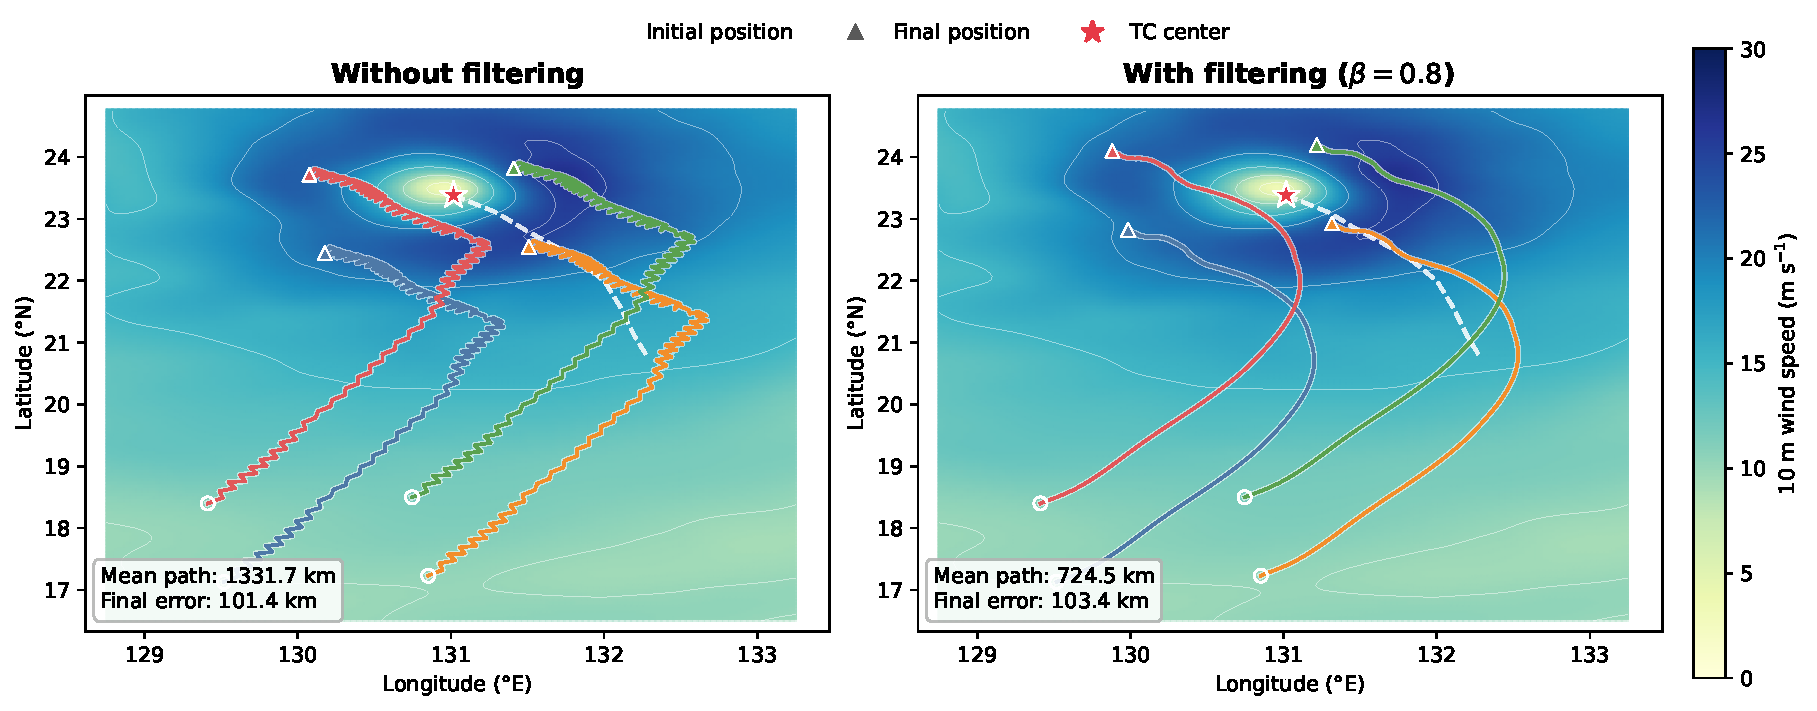
\includegraphics[width=\textwidth]{figures/FigB2_Filter_Path_Comparison.pdf}
\caption{Representative effect of execution-layer filtering on surface paths
for four SUVs under the same trained policy, initial positions, deployment
radius, and KHANUN (2023) segment. The formation center is deployed at a fixed
distance of 400 km from the TC core using a randomly selected bearing. The
left panel uses the raw policy command, whereas the right panel applies the
low-pass filter with $\beta=0.8$. Open circles and triangles mark initial and
final positions, respectively, and the red star marks the TC core.}
\label{fig:filter_path_comparison}
\end{figure*}

\begin{table*}[htbp]
\centering
\caption{Execution-layer low-pass filtering for 4/8/12/16 surface SUVs on 262 held-out segments from 40 unseen TCs in the 400-TC dataset. Each trained actor is evaluated with the filter off and on ($\beta=0.8$) on the same validation episodes. Each entry is the median over validation episodes within a seed, averaged across seeds.}
\label{tab:surface_control_ablations}
\scriptsize
\setlength{\tabcolsep}{2.5pt}
\renewcommand{\arraystretch}{0.9}
\begin{tabular*}{\textwidth}{@{\extracolsep{\fill}}llrrrr@{}}
\toprule
Fleet & Filter & Final tracking error (km) & Path per SUV (km) & Mean speed (m/s) & Maximum speed (m/s) \\
\midrule
4 & Off & 355.4 & 1160.0 & 16.45 & 19.47 \\
4 & On & \textbf{251.3} & \textbf{508.2} & \textbf{8.49} & \textbf{14.25} \\
8 & Off & 324.7 & 1119.5 & 16.11 & 19.47 \\
8 & On & \textbf{277.8} & \textbf{504.7} & \textbf{8.65} & \textbf{15.32} \\
12 & Off & 312.0 & 1019.2 & 14.85 & 19.46 \\
12 & On & \textbf{278.8} & \textbf{497.4} & \textbf{8.52} & \textbf{15.96} \\
16 & Off & 260.2 & 1129.9 & 16.29 & 19.47 \\
16 & On & \textbf{256.1} & \textbf{670.8} & \textbf{11.01} & \textbf{17.97} \\
\bottomrule
\end{tabular*}
\par\smallskip
\parbox{\textwidth}{\footnotesize Final tracking error is the fleet-center-to-TC-core distance at the final time step. Off and on use the same trained actor.}
\end{table*}



\subsection{Subsurface Observation and Comparison with Traditional Planners}
\label{subsec:subsurface_results}
\label{subsec:classical_results}

Before comparing IPPO with non-learned planners, we first isolate its
subsurface performance at each observation depth and propulsion limit.
Appendix Table~\ref{tab:underwater_ippo_main} reports experienced current
speed, geometric coverage, and current-weighted coverage after averaging over
episodes within each training seed and then over ten seeds.

Mean experienced current decreases from 0.534 m/s at the surface to
approximately 0.30 m/s at 60 m under both speed limits. At a fixed depth, the
1.5 and 2.0 m/s policies differ by less than 0.006 m/s in mean experienced
current. The faster envelope mainly expands the sampled region: relative to
1.5 m/s, geometric coverage is 1.18--1.34 times larger and current-weighted
coverage is 1.15--1.30 times larger.

\begin{table*}[t]
\centering
\caption{Comparison with four traditional planning baselines on the held-out
TC segments from the same 400-TC train/test split. Surface values are means
over the 4/8/12/16-SUV fleets, both speed limits, and all five deployment
radii after computing condition medians over validation episodes. Subsurface
values use arithmetic means over all seven depths and both propulsion limits.
Final and mean tracking errors are measured from the fleet center to the TC
core. For surface tracking, lower errors and paths are better. For subsurface
observation, higher current and coverage are better.}
\label{tab:classical_planners}
\small
\resizebox{\textwidth}{!}{%
\begin{tabular}{@{}lrrr@{}}
\toprule
\multicolumn{4}{l}{\textbf{Panel A: surface tracking}}\\
Method & Final tracking error (km) & Mean tracking error (km) & Path per SUV (km)\\
\midrule
IPPO & \textbf{356.2} & \textbf{356.6} & \textbf{462.3} \\
Potential field & 413.4 & 404.2 & 728.8 \\
Receding-horizon A* & 457.2 & 429.4 & 823.9 \\
Lawnmower coverage & 554.7 & 478.4 & 509.1 \\
Information greedy & 466.2 & 429.4 & 528.7 \\
\midrule
\multicolumn{4}{l}{\textbf{Panel B: subsurface observation}}\\
Method & Mean current (m/s) & Geometric coverage (km$^2$) & Current-weighted coverage ($10^3$ m\,s$^{-1}$\,km$^2$)\\
\midrule
IPPO & 0.408 & \textbf{3506} & \textbf{1.599} \\
Potential field & \textbf{0.452} & 2048 & 1.050 \\
Receding-horizon A* & 0.427 & 2310 & 1.097 \\
Lawnmower coverage & 0.408 & 2914 & 1.286 \\
Information greedy & 0.429 & 1549 & 0.739 \\
\bottomrule
\end{tabular}
}
\end{table*}

Appendix Figure~\ref{fig:planner_rendering} shows one matched trajectory
example. Table~\ref{tab:classical_planners} compares IPPO with four traditional
planners. Its surface panel provides matched context, whereas the subsurface
panel is the focus of this section. Across all 40 surface configurations,
IPPO has the lowest final tracking error, mean tracking error, and path length.
It produces a lower final tracking error than potential field in 35 of 40 comparisons
and than each remaining planner in all 40. Its path is shorter than those of
potential field and A* in every comparison and shorter than those of the
lawnmower and information-greedy planners in 26 and 34 of 40 comparisons.
The path advantage over the latter two planners is therefore less uniform than
the final-tracking-error advantage.

For the subsurface task, no planner leads all three metrics. Potential field
has the highest mean experienced current at 0.452 m/s. IPPO has the largest
geometric coverage at 3506 km\(^2\) and the largest current-weighted coverage
\(\mathcal C_{\mathrm w}(z)\). Its mean current of 0.408 m/s is close to that
of the lawnmower planner. IPPO's current-weighted coverage exceeds that of
potential field, A*, lawnmower control, and information-greedy control in all
14 depth--speed settings by factors of 1.41--1.60, 1.39--1.56, 1.17--1.31,
and 1.95--2.28, respectively. Thus, potential field performs better on mean
experienced current, whereas IPPO performs better on geometric and
current-weighted coverage; no method leads all three metrics.

Appendix Table~\ref{tab:planner_stratified} confirms the same pattern after
stratification. IPPO retains the lowest final tracking error and mean tracking error
at every surface deployment radius. Underwater, potential field has the
highest mean current at every depth and IPPO has the largest geometric coverage.

\section{Conclusion}

This study developed and evaluated a shared-action surface IPPO policy and a
parameter-sharing subsurface IPPO policy for
coordinated surface--subsurface tropical-cyclone observation with Blue
Whale-class SUVs. Current and future-upgrade speed settings were evaluated
separately for the surface and subsurface fixed-depth tasks.
Historical atmosphere--ocean reanalysis data, including ERA5 and HYCOM, were
used to construct the simulation environments for SUV reinforcement-learning
training.
Training used 360 TCs, and evaluation used 40 unseen TCs.

At the surface, globally shared wind observations allowed the fleet to approach
the moving TC despite uncertain deployment. The 20 m/s maximum-speed
configuration produced smaller final and mean tracking errors at
every deployment radius, and its final-tracking-error advantage grew with deployment
error. The 12 m/s maximum-speed configuration produced shorter paths and lower
speeds. Action filtering reduced the mean final tracking error at every fleet size
and shortened paths and peak speed. In the eight-SUV formation comparison, the
line formation had the lowest mean final tracking error, the grid had the shortest paths
and widest spacing, and the ring provided a broad sampling footprint and was
retained as the main configuration because no formation was uniformly best. In
the matched surface comparison with four traditional planners, IPPO had the
lowest final and mean tracking errors and generally shorter paths.
It had a lower final tracking error than potential field in most matched cases and
consistently lower error than the other three planners.

At the subsurface, four SUVs sampled one of seven fixed layers using only their local
current histories. The comparison with four traditional planners showed no
single winner across all underwater metrics: potential field obtained the
highest mean current, while IPPO obtained the largest geometric and
current-weighted coverage. Under the same 20 h horizon, increasing the submerged
speed limit from 1.5 to 2.0 m/s expanded the sampled area at every depth. A
faster future SUV offers greater spatial sampling capacity, provided that
endurance and control stability remain feasible.

Nevertheless, several limitations remain. The SUV dynamics are represented by
a simplified horizontal point mass model, and calibrated six-degree-of-freedom
dynamics are not included. The study targets autonomous environmental sensing
and path planning, whereas detailed low-level vehicle control is not modeled.
The retained tail cases also expose two scene-level failure modes. In a
multi-TC environment, another active cyclone can generate a more coherent
local wind signature and divert the fleet from its designated target, as in
the 2012 MARIA--PRAPIROON case. In other cases, weak TC winds and a deployment
far from the core produce insufficient wind-speed contrast for a stable
gradient direction, as in the 2021 OMAIS example. These cases motivate
subsequent work on explicit target encoding, active target disambiguation, and
wind-observation uncertainty.
The main experiments were trained and validated in simulation, and real-vehicle
field experiments were not conducted. Future work can incorporate
six-degree-of-freedom dynamics and low-level control and validate the
algorithms through field experiments in real environments. It should also
address the sim-to-real gap in reinforcement learning. In addition, TC wind
speeds used as observation inputs to the surface policy may be underestimated
in reanalysis datasets, which can affect policy decisions. Future work can use
observed TC wind speeds to fine-tune the existing policy through transfer
learning.

\section*{Code and package availability}
\begin{sloppypar}
The code and processed results are available at\newline
\url{https://github.com/DYHAI/SUV-MARL-TC}. The experiments used Python 3.11,
PyTorch 2.11.0 (CUDA 12.8 build), Stable-Baselines3 2.9.0, and Gymnasium
1.2.2 for policy training; NumPy 2.4.6 and pandas 2.3.3 for numerical and
tabular processing; SciPy 1.17.1, xarray 2026.7.0, netCDF4 1.7.4, and h5py
3.16.0 for analysis and NetCDF processing; and Matplotlib 3.11.1 for
visualization.
\end{sloppypar}

\section*{Acknowledgements}
\begin{sloppypar}
\hyphenpenalty=10000
This project is supported by the National Natural Science Foundation of China
(42530402 and 42227901), the National Natural Science Foundation of China
Youth Science Fund Project (62603673), the China Postdoctoral Science
Foundation (2025M783467), the Project of State Key Laboratory of Satellite
Ocean Environment Dynamics (SOEDZZ2527), and the Innovation Group Project of
Southern Marine Science and Engineering Guangdong Laboratory (Zhuhai)
(311024004).
\end{sloppypar}

\printcredits

\clearpage
\appendix
\onecolumn

\section{Supplementary Observation Results}
\setcounter{figure}{0}
\renewcommand{\thefigure}{A.\arabic{figure}}
\renewcommand{\theHfigure}{A.\arabic{figure}}
\setcounter{table}{0}
\renewcommand{\thetable}{A.\arabic{table}}
\renewcommand{\theHtable}{A.\arabic{table}}

\begin{center}
\centering
\captionof{table}{IBTrACS TC translation speeds for the 400-TC dataset.
The percentages denote the fraction of main-track samples not exceeding
each platform speed. These values describe the speed envelope only;
tracking also depends on deployment offset and tracking duration.}
\label{tab:tc_speed_envelope}
\small
\begin{tabular*}{\textwidth}{@{\extracolsep{\fill}}lrrrrrr@{}}
\toprule
Quantity & P50 & P90 & P95 & P99 & Samples & TCs \\
\midrule
TC translation speed (m s$^{-1}$) & 5.14 & 10.29 & 13.89 & 20.58 & 28,506 & 400 \\
\midrule
Envelope & \multicolumn{2}{c}{Samples within speed} &
\multicolumn{2}{c}{Samples above speed} &
\multicolumn{2}{c}{Interpretation} \\
1.5 m/s submerged & \multicolumn{2}{c}{3.3\%} &
\multicolumn{2}{c}{96.7\%} &
\multicolumn{2}{l}{local sampling, not TC chasing} \\
2.0 m/s submerged & \multicolumn{2}{c}{7.0\%} &
\multicolumn{2}{c}{93.0\%} &
\multicolumn{2}{l}{local sampling, not TC chasing} \\
12 m/s surface & \multicolumn{2}{c}{93.0\%} &
\multicolumn{2}{c}{7.0\%} &
\multicolumn{2}{l}{current-platform scenario} \\
20 m/s surface & \multicolumn{2}{c}{98.8\%} &
\multicolumn{2}{c}{1.2\%} &
\multicolumn{2}{l}{future-upgrade scenario} \\
\bottomrule
\end{tabular*}
\end{center}

\begin{center}
\centering
\captionof{table}{Surface initial-formation comparison for eight SUVs. All four layouts use a mean radius of 100 km. This is a matched single-seed sensitivity study using training seed 0, with formation-center offsets sampled inside an 800 km radius and evaluation without retraining at fixed offsets of 100, 200, 400, 600, and 800 km on the same 262 held-out TC segments. Final tracking error is the fleet-center-to-TC-core distance at the end of the episode, and path is the per-vehicle trajectory length. Entries are medians over validation episodes. Bold entries are the best value in each speed/radius row; error and path are assessed separately. All distances are in km.}
\label{tab:formation_comparison}
\scriptsize
\setlength{\tabcolsep}{1.4pt}
\begin{tabular*}{\textwidth}{@{\extracolsep{\fill}}ccccccccccc@{}}
\toprule
Speed & Train radius & Eval radius & \multicolumn{2}{c}{Ring} & \multicolumn{2}{c}{Line} & \multicolumn{2}{c}{Grid} & \multicolumn{2}{c}{V} \\
\cmidrule(lr){4-5}\cmidrule(lr){6-7}\cmidrule(lr){8-9}\cmidrule(lr){10-11}
(m/s) & (km) & (km) & \makecell{Final tracking\\error} & Path & \makecell{Final tracking\\error} & Path & \makecell{Final tracking\\error} & Path & \makecell{Final tracking\\error} & Path \\
\midrule
12 & 800 & 100 & 210.4 & 284.4 & 184.8 & 330.4 & 295.8 & \textbf{219.3} & \textbf{165.0} & 366.2 \\
12 & 800 & 200 & 228.6 & 317.2 & 202.4 & 364.5 & 317.7 & \textbf{241.2} & \textbf{183.9} & 406.9 \\
12 & 800 & 400 & 312.0 & 364.2 & 295.7 & 409.9 & 408.5 & \textbf{272.8} & \textbf{284.6} & 463.9 \\
12 & 800 & 600 & 445.9 & 383.9 & 452.6 & 408.5 & 542.6 & \textbf{291.4} & \textbf{438.1} & 486.9 \\
12 & 800 & 800 & \textbf{636.5} & 372.4 & 655.6 & 394.1 & 733.5 & \textbf{285.9} & 637.5 & 487.9 \\
\midrule
20 & 800 & 100 & 197.5 & \textbf{356.2} & \textbf{156.4} & 435.3 & 204.7 & 383.2 & 158.1 & 416.6 \\
20 & 800 & 200 & 209.9 & \textbf{404.6} & \textbf{168.0} & 489.5 & 217.7 & 433.7 & 173.8 & 470.6 \\
20 & 800 & 400 & 266.6 & \textbf{502.5} & \textbf{228.4} & 599.5 & 277.7 & 537.7 & 251.8 & 571.0 \\
20 & 800 & 600 & 371.1 & \textbf{571.9} & \textbf{342.1} & 676.6 & 390.6 & 616.4 & 385.3 & 644.7 \\
20 & 800 & 800 & 533.9 & \textbf{607.7} & \textbf{522.0} & 717.2 & 571.1 & 645.5 & 553.3 & 682.8 \\
\bottomrule
\end{tabular*}
\end{center}

\begin{center}
\captionof{table}{IPPO subsurface observation performance at seven depths and
two propulsion limits. For every depth--speed setting, values are means over
validation episodes within each seed and are then averaged over ten training
seeds. Current-weighted coverage is reported in \(10^3\)
m\,s\(^{-1}\)\,km\(^2\). Bold entries denote the larger value within each
depth and metric; equal values remain unbolded.}
\label{tab:underwater_ippo_main}
\small
\begin{tabular*}{\textwidth}{@{\extracolsep{\fill}}rrrrr@{}}
\toprule
Depth (m) & \(V_{\max}\) (m/s) & Mean current (m/s) &
Geometric coverage (km\(^2\)) & Current-weighted coverage \\
\midrule
0  & 1.5 & 0.534 & 3376 & 2.012 \\
0  & 2.0 & 0.534 & \textbf{3968} & \textbf{2.319} \\
\addlinespace[1.5pt]
10 & 1.5 & 0.472 & 3385 & 1.744 \\
10 & 2.0 & \textbf{0.476} & \textbf{4073} & \textbf{2.107} \\
\addlinespace[1.5pt]
20 & 1.5 & 0.444 & 3402 & 1.660 \\
20 & 2.0 & \textbf{0.445} & \textbf{4037} & \textbf{1.956} \\
\addlinespace[1.5pt]
30 & 1.5 & \textbf{0.409} & 3253 & 1.481 \\
30 & 2.0 & 0.408 & \textbf{3895} & \textbf{1.750} \\
\addlinespace[1.5pt]
40 & 1.5 & 0.364 & 2851 & 1.191 \\
40 & 2.0 & \textbf{0.368} & \textbf{3808} & \textbf{1.555} \\
\addlinespace[1.5pt]
50 & 1.5 & 0.324 & 2907 & 1.069 \\
50 & 2.0 & \textbf{0.328} & \textbf{3749} & \textbf{1.374} \\
\addlinespace[1.5pt]
60 & 1.5 & 0.300 & 2818 & 0.959 \\
60 & 2.0 & \textbf{0.305} & \textbf{3559} & \textbf{1.207} \\
\bottomrule
\end{tabular*}
\end{center}

\clearpage
\begin{center}
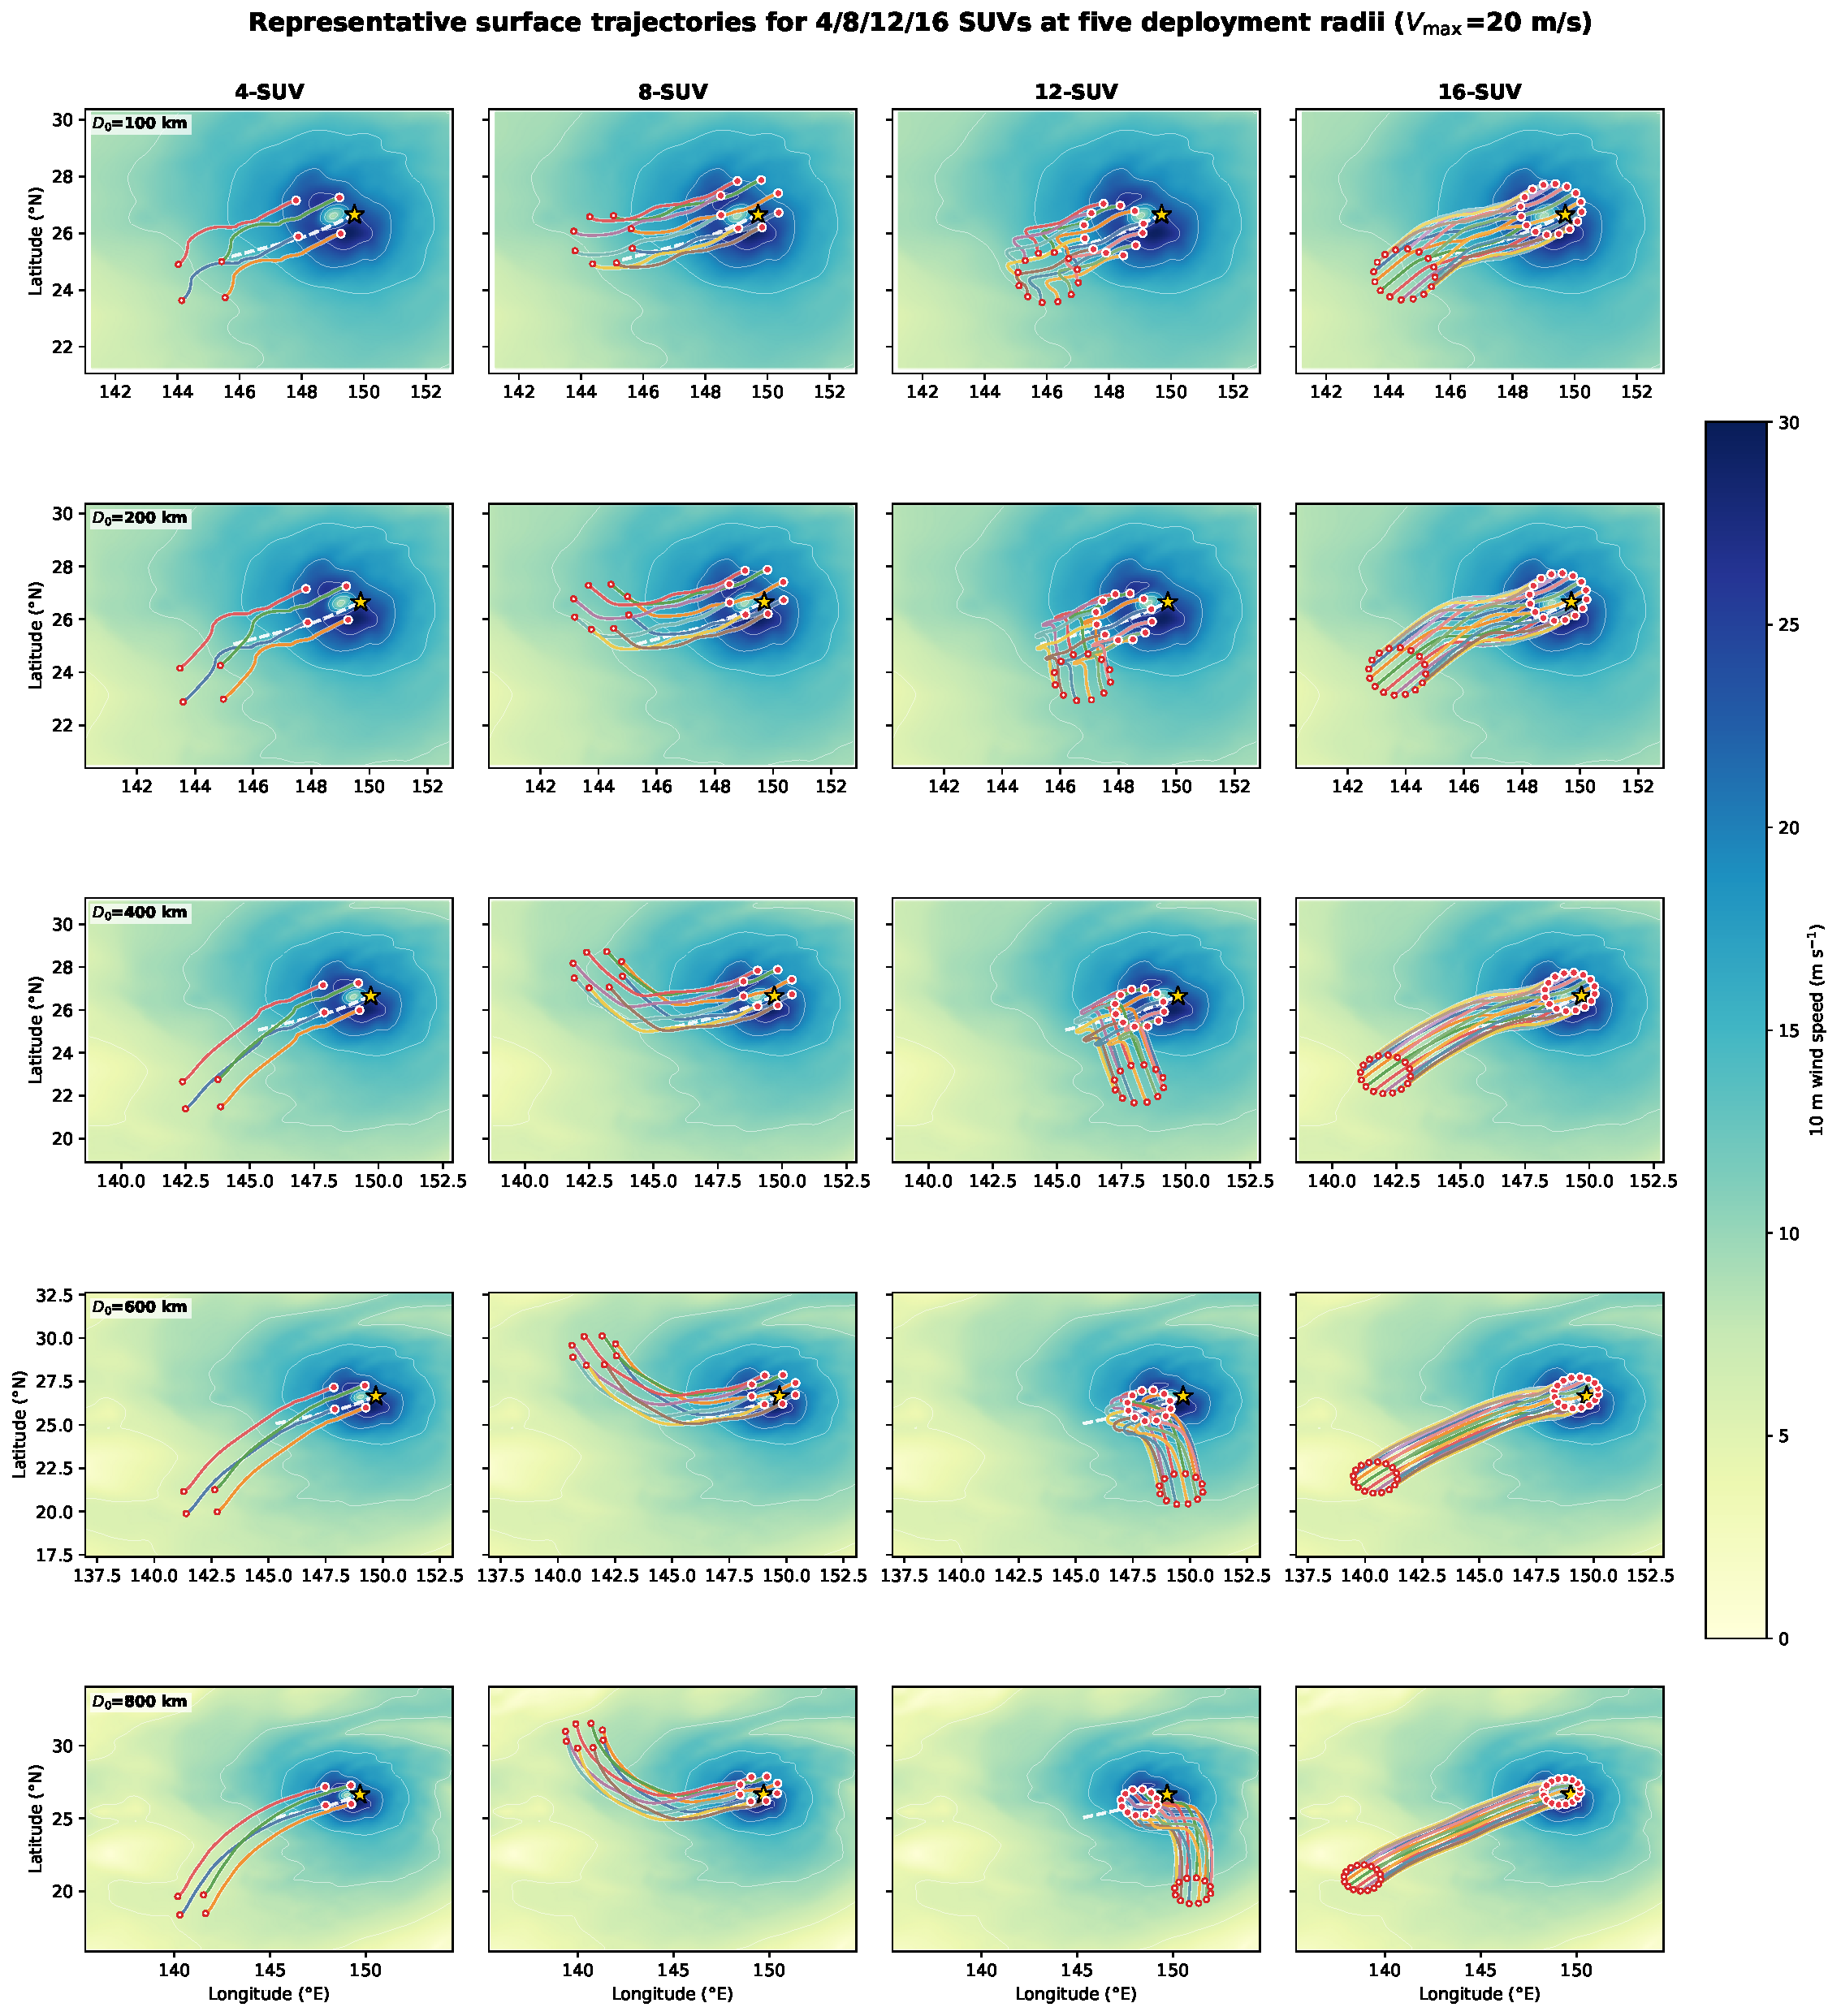
\includegraphics[width=\textwidth]{figures/Fig4_Surface_Trajectory_Matrix.pdf}
\captionof{figure}{Representative KHANUN (2023) trajectories for the final
20 m/s surface policy. Columns show 4-, 8-, 12-, and 16-SUV formations, while
rows show different formation-center deployment radii of 100, 200, 400, 600, and
800 km. For each radius, the formation center is placed at a randomly selected
bearing relative to the TC core. The color background is the spatially
interpolated final-time ERA5 10 m wind-speed field. Thin colored lines are
vehicle trajectories, open circles mark initial positions, small red dots mark
final vehicle positions, and the yellow star marks the TC core at the end of
the episode.}
\label{fig:surface_trajectory_matrix}
\end{center}

\clearpage
\section{Traditional Planner Comparison}
\setcounter{figure}{0}
\renewcommand{\thefigure}{B.\arabic{figure}}
\renewcommand{\theHfigure}{B.\arabic{figure}}
\setcounter{table}{0}
\renewcommand{\thetable}{B.\arabic{table}}
\renewcommand{\theHtable}{B.\arabic{table}}

\begin{center}
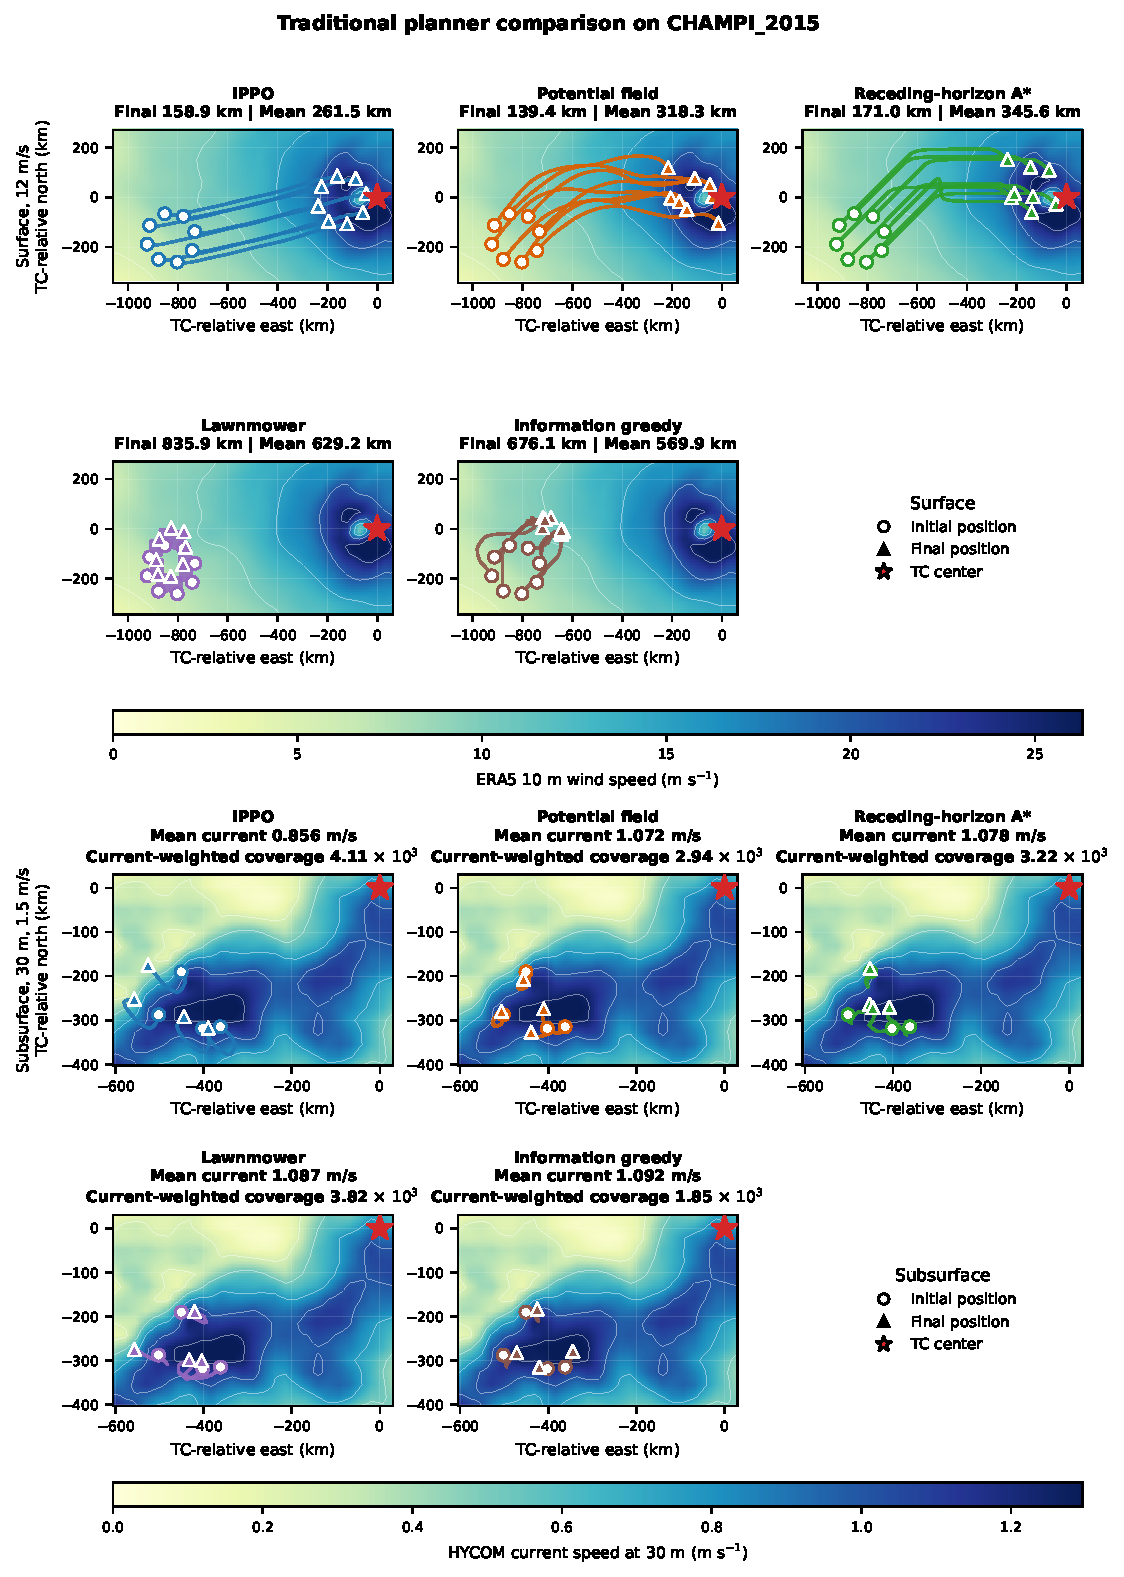
\includegraphics[width=\textwidth,height=0.78\textheight,keepaspectratio]
  {figures/Fig7_Traditional_Planner_Rendering.pdf}
\small
\captionof{figure}{Comparison between IPPO and the four traditional planners on
the same CHAMPI segment. The upper two rows show 12 m/s surface trajectories
over the ERA5 10 m wind-speed field. The lower two rows show 1.5 m/s subsurface
trajectories at 30 m over the HYCOM current-speed field. All methods use the
same initial deployment. The surface formation center is deployed at a distance
of 400 km from the TC core, and the subsurface SUVs are initialized
within a 200 km radius of the TC core. Panel titles report final and mean
tracking errors for the surface task and mean experienced current
for the subsurface task. Open
circles mark initial positions, triangles mark final positions, and the red
star marks the TC core.}
\label{fig:planner_rendering}
\end{center}

\begin{center}
\captionof{table}{Distance and observation metrics for the traditional planner comparison on the held-out TC segments. Panel A reports episode-median final and mean tracking errors by deployment radius, averaged over the four fleet sizes and both speed limits. Panel B reports episode-mean experienced current speed, geometric coverage, and current-weighted coverage at each depth, averaged over the two propulsion limits. Current-weighted coverage is reported in \(10^3\) m\,s\(^{-1}\)\,km\(^2\). For surface tracking, lower errors and paths are better. For subsurface observation, higher current and coverage are better.}
\label{tab:planner_stratified}
\footnotesize
\setlength{\tabcolsep}{4pt}
\renewcommand{\arraystretch}{1.04}
\begin{tabular*}{\textwidth}{@{\extracolsep{\fill}}llrrrrr@{}}
\toprule
\multicolumn{7}{l}{\textbf{Panel A: surface tracking metrics}}\\
Radius & Metric & IPPO & PF & A* & Lawn & Greedy\\
\midrule
100 km & Final tracking error (km) & \textbf{220.8} & 290.4 & 325.8 & 366.1 & 295.2 \\
 & Mean tracking error (km) & \textbf{170.6} & 229.9 & 250.5 & 232.9 & 212.0 \\
\addlinespace[1.5pt]
200 km & Final tracking error (km) & \textbf{236.1} & 295.4 & 330.0 & 394.5 & 310.7 \\
 & Mean tracking error (km) & \textbf{197.6} & 248.5 & 267.1 & 285.9 & 244.5 \\
\addlinespace[1.5pt]
400 km & Final tracking error (km) & \textbf{304.0} & 353.5 & 394.9 & 504.5 & 405.1 \\
 & Mean tracking error (km) & \textbf{303.0} & 343.0 & 367.4 & 441.8 & 374.5 \\
\addlinespace[1.5pt]
600 km & Final tracking error (km) & \textbf{423.9} & 476.1 & 527.6 & 661.2 & 560.1 \\
 & Mean tracking error (km) & \textbf{460.8} & 505.1 & 536.7 & 621.7 & 559.1 \\
\addlinespace[1.5pt]
800 km & Final tracking error (km) & \textbf{596.1} & 651.8 & 707.6 & 847.4 & 759.8 \\
 & Mean tracking error (km) & \textbf{650.8} & 694.4 & 725.0 & 809.7 & 756.7 \\
\addlinespace[1.5pt]
\midrule
\multicolumn{7}{l}{\textbf{Panel B: subsurface metrics by depth}}\\
Depth & Metric & IPPO & PF & A* & Lawn & Greedy\\
\midrule
0 m & Mean experienced current (m/s) & 0.534 & \textbf{0.577} & 0.548 & 0.536 & 0.551 \\
 & Geometric coverage (km$^2$) & \textbf{3672} & 2214 & 2445 & 3067 & 1579 \\
 & Current-weighted coverage & \textbf{2.335} & 1.443 & 1.467 & 1.756 & 0.956 \\
\addlinespace[1.5pt]
10 m & Mean experienced current (m/s) & 0.474 & \textbf{0.515} & 0.489 & 0.472 & 0.492 \\
 & Geometric coverage (km$^2$) & \textbf{3729} & 2189 & 2414 & 3020 & 1620 \\
 & Current-weighted coverage & \textbf{1.955} & 1.249 & 1.284 & 1.513 & 0.876 \\
\addlinespace[1.5pt]
20 m & Mean experienced current (m/s) & 0.444 & \textbf{0.486} & 0.462 & 0.444 & 0.464 \\
 & Geometric coverage (km$^2$) & \textbf{3720} & 2152 & 2388 & 2987 & 1632 \\
 & Current-weighted coverage & \textbf{1.877} & 1.153 & 1.204 & 1.415 & 0.835 \\
\addlinespace[1.5pt]
30 m & Mean experienced current (m/s) & 0.409 & \textbf{0.452} & 0.429 & 0.410 & 0.431 \\
 & Geometric coverage (km$^2$) & \textbf{3574} & 2105 & 2329 & 2939 & 1588 \\
 & Current-weighted coverage & \textbf{1.624} & 1.039 & 1.104 & 1.291 & 0.754 \\
\addlinespace[1.5pt]
40 m & Mean experienced current (m/s) & 0.366 & \textbf{0.412} & 0.386 & 0.368 & 0.391 \\
 & Geometric coverage (km$^2$) & \textbf{3330} & 1999 & 2273 & 2876 & 1542 \\
 & Current-weighted coverage & \textbf{1.469} & 0.894 & 0.970 & 1.141 & 0.666 \\
\addlinespace[1.5pt]
50 m & Mean experienced current (m/s) & 0.326 & \textbf{0.374} & 0.349 & 0.327 & 0.351 \\
 & Geometric coverage (km$^2$) & \textbf{3328} & 1876 & 2200 & 2803 & 1470 \\
 & Current-weighted coverage & \textbf{1.246} & 0.750 & 0.848 & 0.986 & 0.575 \\
\addlinespace[1.5pt]
60 m & Mean experienced current (m/s) & 0.302 & \textbf{0.350} & 0.325 & 0.301 & 0.324 \\
 & Geometric coverage (km$^2$) & \textbf{3189} & 1799 & 2120 & 2702 & 1410 \\
 & Current-weighted coverage & \textbf{1.092} & 0.658 & 0.765 & 0.877 & 0.519 \\
\bottomrule
\end{tabular*}
\end{center}

\clearpage
\section{IPPO Algorithm Parameters}\label{app:parameters}

\setcounter{table}{0}
\renewcommand{\thetable}{C.\arabic{table}}
\renewcommand{\theHtable}{C.\arabic{table}}

Table~\ref{tab:reward_parameters} summarizes the reward, action-filter, and
safety parameters used in the surface and underwater experiments.
Table~\ref{tab:ippo_hyperparams} lists the shared IPPO network and training
hyperparameters.

% ============================================================
% Table A.2: Merged reward and safety parameters
% ============================================================
\begin{center}
\small
\renewcommand{\arraystretch}{1.0}
\captionof{table}{Surface and subsurface reward, action-filter, and
coastal-safety parameters used in the final experiments.}
\label{tab:reward_parameters}
\resizebox{\textwidth}{!}{%
\begin{tabular}{@{}p{0.18\textwidth}p{0.12\textwidth}p{0.15\textwidth}p{0.45\textwidth}@{}}
\toprule
Parameter & Symbol & Value & Description and applicable task \\
\midrule
\multicolumn{4}{l}{\textbf{Panel A: surface reward and controller parameters}} \\
Proximity-cost distance cap & $D_{\max}$ & 300 km &
Distance cost is capped at 300 km to prevent excessively large gradients
from distant initial deployments. \\
Distance normalization scale & $D_{\mathrm{scale}}$ & 100 km &
Normalization scale used by the proximity and radius-excess reward terms. \\
Near-center threshold & $d_{\mathrm{near}}$ & 100 km &
Threshold defining the discrete near-center bonus. \\
Near-center bonus & $b_{\mathrm{near}}$ & 1.0 &
Bonus assigned when an SUV is within 100 km of the TC core. \\
Radius-excess threshold & $R_{\mathrm{form}}$ & 100 km &
Reference radius used by the additional distance penalty beyond 100 km. \\
Radius-excess weight & $W_{\mathrm{form}}$ & 1.0 &
Weight of the penalty applied when an individual SUV is farther than 100 km
from the TC core. \\
Action-change weight & $\lambda_u$ & 0.05 &
Weight of the squared action change
$\|\bar{\mathbf{a}}_{i,k}-\bar{\mathbf{a}}_{i,k-1}\|_2^2$ between
successive executed commands. \\
Action-filter coefficient & $\beta$ & 0.8 &
Coefficient of
$\mathbf{a}_k^{\mathrm{filt}}=
(1-\beta)\mathbf{a}_k^{\mathrm{raw}}
+\beta\mathbf{a}_{k-1}^{\mathrm{filt}}$.
This is a controller setting and is not included in the reward. \\
Surface reward clipping range & $[r_{\min},r_{\max}]$ & $[-5,2]$ &
Clipping range applied to the team-averaged surface reward. \\

\midrule
\multicolumn{4}{l}{\textbf{Panel B: underwater IPPO parameters}} \\
Current-speed normalization & $V_{\mathrm{norm}}$ & 1.0 m/s &
Current-intensity reward is implemented as
$\min(\|\mathbf{u}\|/V_{\mathrm{norm}},R_{\max})$. \\
Current-reward cap & $R_{\max}$ & 2.0 &
Upper bound of the normalized current-speed reward. \\
Downstream-alignment weight & $\beta_{\parallel}$ & 0.5 &
Weight of the positive propulsion--current alignment term. \\
Normalized action-magnitude weight & $\lambda_a$ & 0.05 &
Penalizes the squared magnitude of the normalized propulsion command. This
term regularizes the controller response. \\
Underwater reward clipping range & $[r_{\min},r_{\max}]$ & $[-5,5]$ &
Clipping range applied to the team-averaged underwater reward during IPPO
training. \\

\midrule
\multicolumn{4}{l}{\textbf{Panel C: coastal-safety parameters by stage}} \\
Land penalty & $P_{\mathrm{land}}$ & 20 &
Penalty applied when an SUV enters a land cell in either stage. \\
Nearshore buffer distance & $D_{\mathrm{buf}}$ & 100 km &
Width of the soft nearshore penalty buffer in both stages. \\
Nearshore penalty weight & $W_b$ & 8.0 &
Maximum soft-penalty weight within the 100 km nearshore buffer in either
stage. \\
Minimum deployment offshore distance & $D_{\mathrm{deploy}}$ & 100 km &
Minimum coastline distance required by offshore-only rejection sampling during
surface deployment; it is not applied to subsurface initialization. \\
Action-filter safety margin & $D_{\mathrm{filter}}$ & 100 km &
Surface-stage distance below which the onshore component of the commanded
action is removed. The subsurface comparison does not use this filter. \\
\bottomrule
\end{tabular}}
\end{center}

\clearpage

% ============================================================
% Table A.3: IPPO hyperparameters
% ============================================================
\noindent\begin{minipage}{\textwidth}
\centering
\fontsize{7.6pt}{8.6pt}\selectfont
\captionof{table}{Shared-action and parameter-sharing IPPO network, training, and deployment
hyperparameters used in the final surface and subsurface experiments.}
\label{tab:ippo_hyperparams}
\resizebox{\textwidth}{!}{%
\begin{tabular}{@{}p{0.18\textwidth}p{0.13\textwidth}p{0.17\textwidth}p{0.42\textwidth}@{}}
\toprule
Parameter & Symbol & Value & Description \\
\midrule
Algorithm & -- & PPO &
Stable-Baselines3 PPO with one shared surface formation action and independent
per-agent action sampling underwater. \\
Optimizer & -- & Adam &
Adam optimizer used for the actor and critic parameters. \\
Policy network & -- & $2\times256$ MLP &
Actor: Linear($d_{\mathrm{obs}},256$)--Tanh--
Linear($256,256$)--Tanh--Linear($256,d_{\mathrm{act}}$). \\
Value network & -- & $2\times256$ MLP &
Critic: Linear($d_{\mathrm{obs}},256$)--Tanh--
Linear($256,256$)--Tanh--Linear($256,1$).
Surface training uses one fleet value; underwater training sums per-agent values. \\
Per-agent observation dimension & $d_{\mathrm{obs}}$ & 16/28/40/52; 19 &
Surface observations for 4/8/12/16 SUVs are 16/28/40/52,
respectively. The
four-SUV underwater IPPO evaluation uses
$d_{\mathrm{obs}}=19$. \\
Surface observation & -- & Wind at 10 m above sea level &
Using ideal surface communication, the fleet forms one shared vector of wind
speed and components at 10 m above the sea surface from all SUVs. The common
surface policy query also receives the common normalized ground velocity and
$[\cos\psi,\sin\psi]$. \\
Underwater observation & -- & Current only &
With no inter-vehicle communication, the active IPPO policy observes only
its own local current speed and components at the assigned ocean depth, together
with a five-frame history, its own normalized propulsion velocity, and
$[\cos\psi,\sin\psi]$. \\
Action dimension & $d_{\mathrm{act}}$ & 2 per fleet; 2 per SUV underwater &
The surface policy emits one continuous east--north joint formation command in
$[-1,1]^2$ and applies it to every SUV. Underwater, each SUV receives its
own two-dimensional command. Circular projection enforces the speed bound. \\
Surface formation constraint & -- & Hard shared action &
All surface SUVs execute the same action and retain fixed initial relative
offsets throughout an episode. \\
Rollout length & $n_{\mathrm{steps}}$ & 2048 &
Number of steps collected per environment before each PPO update. \\
Mini-batch size & $B$ & 256 &
Mini-batch size used during each gradient update. \\
Optimization epochs & $N_{\mathrm{epochs}}$ & 10 &
Number of passes over each rollout. \\
Learning rate & $\alpha$ & $3\times10^{-4}$ &
Adam learning rate used by the actor and critic. \\
Discount factor & $\gamma$ & 0.99 &
Reward discount factor. \\
GAE parameter & $\lambda_{\mathrm{GAE}}$ & 0.95 &
Generalized advantage estimation applied to the team-average reward. \\
Policy clipping range & $\epsilon$ & 0.2 &
Clipping range of the PPO probability ratio. \\
Value clipping range & $\epsilon_v$ & 0.2 &
Clipping range of the value-function update. \\
Entropy coefficient & $c_{\mathrm{ent}}$ & 0.01 &
Entropy regularization coefficient. \\
Value-loss coefficient & $c_v$ & 0.5 &
Weight of the value-function loss. \\
Maximum gradient norm & $g_{\max}$ & 0.5 &
Global gradient clipping threshold. \\
Training steps & $T$ & $2\times10^6$ &
Nominal environment steps per training run. \\
Training seeds & -- & 0--9 &
Ten random seeds for each selected surface or underwater IPPO configuration. \\
Surface training forecast-error radius & $R_{\mathrm{train}}$ & 0--800 km &
The candidate surface formation-center radial offset is sampled uniformly in
\([0,800]\) km, with a uniformly sampled bearing. This models the assumed
upper bound of TC track-forecast error; offshore-only rejection sampling is
then applied as part of the safety layer. \\
Surface validation center offsets & $R_{\mathrm{test}}$ &
100/200/400/600/800 km &
Fixed surface formation-center offsets with random bearings, evaluated without
retraining. These values represent increasing track-forecast displacement. \\
Underwater initialization radius & $R_{0,\mathrm{u}}$ & $\leq$200 km &
At the end time of each surface segment, the separate subsurface episode
initializes four vehicles with radial offsets sampled uniformly in
\([0,200]\) km and uniformly sampled bearings. Surface endpoint positions are
not transferred. The 0--800 km forecast-error protocol is surface-only. \\
Decision interval & $\Delta t$ & 10 min &
Environmental observation and action interval. \\
Initial formation mean radius & $R_{\mathrm{form}}$ & 100 km &
Ring, line, grid, and V layouts are normalized to the same mean radius. \\
Surface fleet sizes & $N$ & 4/8/12/16 &
Number of SUVs in the final surface configurations. \\
Underwater fleet size & $N$ & 4 &
Number of SUVs in each underwater comparison case. \\
Underwater depths below the sea surface & $z$ &
0/10/20/30/40/50/60 m &
Seven ocean-current observation depths used in the final subsurface matrix. \\
Underwater methods & -- & IPPO; PF; A*; lawn; greedy &
IPPO and four traditional planners evaluated on the same episodes and
deployments. \\
Underwater duration & $H$ & 20 h &
Fixed simulation horizon for the final subsurface comparison; this is not an
endurance specification. \\
Surface ground-speed limits & $V_{\max}^{\mathrm{s}}$ & 12 or 20 m/s &
Two commanded ground-speed envelopes; these are modeled scenarios,
not independently measured certifications. \\
Submerged speed limits & $V_{\max}^{\mathrm{u}}$ & 1.5 or 2.0 m/s &
Two propulsion-speed limits after unit-disk action projection
used for underwater IPPO evaluation. \\
Compute device & -- & CPU &
All reported IPPO experiments were trained on CPU. \\
\bottomrule
\end{tabular}}
\end{minipage}

\clearpage
\clearpage
\twocolumn
\bibliographystyle{elsarticle-num}
\bibliography{main}



%\vskip3pt

% \bio{}
% Author biography without author photo.
% Author biography. Author biography. Author biography.
% Author biography. Author biography. Author biography.
% Author biography. Author biography. Author biography.
% Author biography. Author biography. Author biography.
% Author biography. Author biography. Author biography.
% Author biography. Author biography. Author biography.
% Author biography. Author biography. Author biography.
% Author biography. Author biography. Author biography.
% Author biography. Author biography. Author biography.
% \endbio

% \bio{figs/pic1}
% Author biography with author photo.
% Author biography. Author biography. Author biography.
% Author biography. Author biography. Author biography.
% Author biography. Author biography. Author biography.
% Author biography. Author biography. Author biography.
% Author biography. Author biography. Author biography.
% Author biography. Author biography. Author biography.
% Author biography. Author biography. Author biography.
% Author biography. Author biography. Author biography.
% Author biography. Author biography. Author biography.
% \endbio

% \bio{figs/pic1}
% Author biography with author photo.
% Author biography. Author biography. Author biography.
% Author biography. Author biography. Author biography.
% Author biography. Author biography. Author biography.
% Author biography. Author biography. Author biography.
% \endbio

\end{document}
